\pdfoutput=1
\documentclass[a4paper]{amsart}
\usepackage{knottedStyle,knottedMacros}



\title{Knotted families of (long) knots from graspers}


\author{Danica Kosanovi\'c}
\address{ETH Z\"urich, Department of Mathematics, R\"amistrasse 101, 8092 Z\"urich, Switzerland}
\email{danica.kosanovic@math.ethz.ch}


\date{\today}


\begin{document}

\begin{abstract}
    For any smooth manifold $M$ of dimension $d\geq4$ we construct explicit classes in homotopy groups of spaces of embeddings of either an arc or a circle into $M$, in every degree that is a multiple of $d-3$, and show that they are detected in the Taylor tower of Goodwillie and Weiss.
\end{abstract}

\maketitle

\begin{spacing}{0.5}
    \tableofcontents
\end{spacing}


\section{Introduction}\label{sec:intro}

Given smooth manifolds $C$ and $M$ let $K\colon C\hra M$ be a neat smooth embedding. This means that $K$ is a smooth injective map with injective derivative at each point, $K(C)$ intersects $\partial M$ transversely and precisely in $K(\partial C)$, and we assume that the boundary condition $K|_{\partial C}$ is fixed. 

Let $\D^k$ denote the unit ball in $\R^k$. The trefoil knot $T\colon\D^1\hra\D^3$ can be obtained from the standard embedding $\u\colon\D^1\hra\D^3$, called the unknot, by the following operation. Consider the meridians $m_1,m_2\colon\S^1\hra\D^3\sm\u(\D^1)$ to $\u$ at two different points, then replace a subarc of $\u$ by the arc describing the commutator $[m_1,m_2]\coloneqq m_1m_2m_1^{-1}m_2^{-1}$, as on the left of Figure~\ref{fig:Borr}. Equivalently, pick three subarcs of $\u$ and connect sum them into the Borromean rings, see the right hand side of Figure~\ref{fig:Borr}. This operation is called the Gusarov--Habiro \emph{clasper surgery} on $\u$ of degree $n=2$ \cite{Gusarov-main,Gusarov,Habiro}. In general, a surgery of degree $n\geq1$ uses $n-1$ copies of the Borromean rings and $n+1$ subarcs of $\u$, and follows a shape of a planar rooted binary tree with $n$ leaves. For $n=1$ clasper surgery is simply a crossing change: ambiently connect sum a subarc of $\u$ into a meridian of $\u$.

% Figure environment removed
In other dimensions certain analogues of clasper surgery have been considered. For example, for any $k\geq2$ one can start with the standard embedding $\u\colon\D^{4k-1}\hra\D^{6k}$, pick two meridians $m_1,m_2\colon\S^{2k}\hra\D^{6k}\sm\u(\D^{4k-1})$, defined as the boundaries of the normal disks at two points of $\u(\D^{4k-1})$, and consider their Whitehead product $[m_1,m_2]\colon\S^{4k-1}\to\S^{2k}\vee\S^{2k}\to\D^{6k}\sm\u(\D^{4k-1})$. This is defined by postcomposing with $m_1\vee m_2$ the universal Whitehead product $\S^{4k-1}\to\S^{2k}\vee\S^{2k}$, which is the attaching map of the top $4k$-cell in $\S^{2k}\times\S^{2k}$. It turns out that $[m_1,m_2]$ is homotopic to an embedding (see Section~\ref{subsec:Haefliger}):
\[
    [m_1,m_2]_{emb}\colon\S^{4k-1}\hra\D^{6k}\sm\u(\D^{4k-1}).
\]
Thus, we can tube $\u$ into the sphere $[m_1,m_2]_{emb}$ (i.e.\ ambiently connect sum them), to obtain a new embedding $T\colon\D^{4k-1}\hra\D^{6k}$. This is precisely the trefoil of Haefliger~\cite{Haefliger}, which generates the group of isotopy classes $\pi_0\Embp(\D^{4k-1},\D^{6k})\cong\Z$, as he showed in \cite{Haefliger2} (note that since codimension is $2k+1>2$ by Zeeman~\cite{Zeeman} this group is trivial in the $\mathsf{PL}$ and $\mathsf{Top}$ categories!). Other analogues of clasper surgery appear in Koschorke's work in the context of link maps, see for example~\cite{Koschorke-arbitrary}, and more recently, in the construction of Watanabe~\cite{Watanabe} of nontrivial classes in homotopy groups of the space of diffeomorphisms of a disk of any dimension. See Section~\ref{subsec:related-work}.

In this paper we generalise clasper surgery in another way, namely, for embeddings of a $1$-dimensional source $C$ into a smooth manifold $M$ of dimension $d\geq4$, with a fixed boundary condition. However, instead of studying as above the set of isotopy classes of embeddings, which is the set $\pi_0\Embp(C,M)$ of path components, we study \emph{higher homotopy groups} $\pi_k\Embp(C,M)$, $k\geq1$, where $\u\colon C\hra M$ is an arbitrary basepoint which we omit from the notation. Thus, a nontrivial ``knot'' is now a nonzero homotopy class, represented by a $k$-parameter family of embeddings of $C$ into $M$ which cannot be trivialised through such families. In other words, all embeddings are isotopic to $\u$, but the family cannot be homotoped to the family $\const_\u$ constantly equal to $\u$.

In this setting a meridian of $\u$ (the boundary of a normal disk) is a sphere of dimension $d-2$, so the Whitehead product of $n$ meridians is a sphere of dimension $n(d-3)+1$ (we will actually use the equivalent Samelson product, see Section~\ref{subsec:Samelson}). We can foliate this sphere by embedded circles, and then ambiently connect sum a fixed subarc of $\u$ into each of these circles, to obtain an $n(d-3)$-parameter family of embeddings of $C$, so an element of $\pi_{n(d-3)}\Embp(C,M)$. We make this idea precise in the form of \emph{grasper surgery}, which generalises clasper surgery to all embedding spaces with $1$-dimensional source.

In particular, for grasper surgery of degree $n=1$ we connect sum $\u$ with the circles foliating its meridian. Note that we have to pick an arc guiding a subarc of $\u$ into the vicinity of the meridian, and this choice is up to isotopy determined by a fundamental group element $g\in\pi_1M$, since $d\geq4$. There is a crossing change homotopy from the resulting family back to $\const_\u$ through immersions, by foliating the meridian ball. This defines a realisation map into the relative homotopy group:
\begin{equation}\label{eq:realmap1}
    \realmap_1\colon \Z[\pi_1M]\ra
    \pi_{d-2}\big(\Imm_\partial(C,M),\Embp(C,M)\big).
\end{equation}
This map is an isomorphism for $C$ connected (that is, $C=\D^1$ or $C=\S^1$), as we elaborate in the next paragraph. By general position such relative homotopy groups vanish in degrees $k<d-2$, implying that $\pi_k\Embp(C,M)\cong \pi_k\Imm(C,M)$ for $k<d-3$. Thus, $\pi_{d-3}$ is the lowest homotopy group that can distinguish embeddings from immersions, and we claim the difference between them (i.e.\ the kernel of the surjection $\pi_{d-3}\Embp(C,M)\sra \pi_{d-3}\Imm(C,M))$ is a quotient of $\Z[\pi_1M]$.

The inverse of $\realmap_1$ is an explicit map $\Dax$ coming from the work of Dax \cite{Dax}, as shown in \cite{KT-highd}, and in \cite{Gabai-disks} for $d=4$, and \cite{K-Dax} for $C=\S^1$. Equivalently -- and relevantly for this paper, $\Dax=\evrel_2$ is the map to the second layer of the Taylor tower constructed by Goodwillie and Weiss~\cite{Weiss}. This is a tower of spaces $\cdots\to T_{n+1}(C,M)\to T_n(C,M)\to\cdots$ with maps
\[
    \ev_n\colon \Embp(C,M)\ra T_n(C,M),
    \quad n\geq1,
\]
so that on relative homotopy groups one has the induced map
\[
    \evrel_{n+1}\colon\pi_k\big(T_n(C,M),\Embp(C,M)\big)\ra \pi_k\big(T_n(C,M),T_{n+1}(C,M)\big).
\]
The latter group is trivial for $1\leq k\leq n(d-3)$ and in \cite{K-thesis-paper} we defined an explicit isomorphism
\begin{equation}\label{eq:Lie}
    \pi_{n(d-3)+1}\big(T_n(C,M),T_{n+1}(C,M)\big)\overset{\cong}{\ra}\Lie_{\pi_1M}(n),
\end{equation}
with the group of $\pi_1M$-decorated Lie trees $\Lie_{\pi_1M}(n)$: this is the quotient by the antisymmetry $(\AS)$ and Jacobi relations $(\IHX)$ of the free abelian group $\Z[\Tree_{\pi_1M}(n)]$ generated by the set $\Tree_{\pi_1M}(n)$ of planar rooted trivalent trees with $n$ leaves decorated by elements of $\pi_1M$, see Section~\ref{subsec:trees}.



\begin{theorem}\label{thm:main}
    Let $C$ be equal to $\D^1$ or $\S^1$ and $M$ be any compact smooth manifold with boundary, $\dim M=d\geq4$. For any $n\geq1$ there is an explicit homomorphism
    \[
        \realmap_n\colon\Lie_{\pi_1M}(n)\ra\pi_{n(d-3)+1}\big(T_n(C,M),\Embp(C,M)\big)
    \]
    of abelian groups, given by ``grasper surgery of degree $n$'', such that 
    \[
    \evrel_{n+1}\circ\realmap_n=\Id_{\Lie_{\pi_1M}(n)}.
    \]
\end{theorem}
The essence of the theorem is the compatibility of a priori very different $n$-fold brackets. Namely, on one hand the generators of \eqref{eq:Lie} come from $n$-fold Whitehead brackets of $(d-1)$-spheres (of configurations in $\Conf(M)$ where one point goes around another one locally), whereas degree $n$ graspers involve certain brackets of $(d-2)$-spheres (which are meridians of $\u$). Thus, the proof calls for a thorough geometric understanding of the evaluation maps $\ev_n$, which we obtain using the reduced punctured knots model $\rpT_n(M)$ developed in \cite{KT-rpn}. The two viewpoints fit together via a sort of suspension operation, cf.\ Lemma~\ref{lem:suspensions}.
\begin{cor}\label{cor:main}
    For every linear combination $F$ of trees from the set $\Tree_{\pi_1M}(n)$ there is a family $\realmap_n(F)\colon\S^{n(d-3)}\to\Embp(C,M)$, which is homotopic to $\const_\u$ if and only if $F$ belongs to the linear combination of $(\AS)$ and $(\IHX)$ relations and the image of $\delta_n\colon\pi_{n(d-3)+1}T_n(C,M)\to\Lie_{\pi_1M}(n)$.
    Moreover, the nontriviality of $\realmap_n(F)$ is first detected in $\pi_{n(d-3)}T_k(C,M)$ for $k=n+1$. 
\end{cor}

The homomorphism $\delta_n$ comes from the natural map from the absolute to the relative homotopy group, and its image can be identified with the union of images of the differentials in a spectral sequence computing the homotopy groups of $T_k(C,M)$, $k\geq1$. This spectral sequence has been studied extensively, see Section~\ref{subsec:related-work} for some references.


    In the proof of Corollary~\ref{cor:main} we use the Goodwillie--Klein--Weiss convergence theorem~\cite{GKW,GKmultiple}, which says that $\evrel_{n+1}$ is an isomorphism for $1\leq k\leq (n+1)(d-3)$, cf.\ Theorem~\ref{thm:rpn} below.
    However, in the proof of Theorem~\ref{thm:main} we do not use that result, so this independently shows the surjectivity of $\evrel_{n+1}$, and thus of $\pi_{n(d-3)}\ev_{n+1}$ by induction. See also Questions~\ref{quest:real-map-all-deg} and \ref{quest:reprove-GKW}.



\subsection{Comments}

Let us give a few comments on the proof of Theorem~\ref{thm:main}, referring to Section~\ref{subsec:overview} below for a more detailed summary. The case $d=3$ was proven in \cite{K-thesis-paper}, and a proof for $d\geq4$ was hinted in Remark~1.10 of that paper. Here we carry out all the details, and actually give a slightly simpler proof. For a decorated tree $\Gamma^{g_{\ul{n}}}$, we will:
\begin{enumerate}
    \item
define a knotted family $\realmap_n(\Gamma^{g_{\ul{n}}})\colon\S^{n(d-3)}\to\Embp(C,M)$, using a family $\mu_{\Gamma,d}$ of arcs in $\ball^d$ and any grasper $\TG_n\colon \ball^d\hra M$ of degree $n$ relative to $\u$, decorated by $g_{\ul{n}}=(g_1,\dots,g_n)$;
    \item 
exhibit a homotopy from $\ev_n\realmap_n(\Gamma^{g_{\ul{n}}})$ to $\ev_n(\const_\u)$ through maps $\S^{n(d-3)}\to T_n(C,M)$, using a multi-family $\mu^\star_{\Gamma,d}$ of arcs in $\ball^d$;
    \item 
check that $\evrel_{n+1}$ of the resulting relative homotopy class is equal to $[\Gamma^{g_{\ul{n}}}]\in\Lie_{\pi_1M}(n)$.
\end{enumerate}

A \emph{grasper} of degree $n$ is simply an embedding $\TG_n\colon\ball^d\hra M$, which is disjoint from $\partial M$, and which intersects the basepoint knot $\u$ in fixed intervals
\begin{equation}\label{eq:G-condition}
    \TG_n(\ball^d)\cap\u(C)=\u(J_i)=\TG_n(a_i)
\end{equation}
for some fixed arcs $a_i\colon\D^1\hra\ball^d$ with $0\leq i\leq n$.
The family $\mu_{\Gamma,d}$ of reimbeddings of the arc $a_0$ can be viewed as the \emph{universal iterated Whitehead product} of the shape $\Gamma$ and dimension $d$, whereas $\realmap_n(\Gamma^{g_{\ul{n}}})$ is the mentioned \emph{embedded version of the Whitehead product} according to $\Gamma^{g_{\ul{n}}}$ of meridian spheres for $\u$. Thus,  $\mu_{\Gamma,d}$ plays the role of a clasper, while $\realmap_n(\Gamma^{g_{\ul{n}}})$ generalises clasper surgery.

When introducing this notion we are inspired by \emph{gropes} of Conant and Teichner~\cite{CT1} and \emph{claspers} of Gusarov and Habiro \cite{Gusarov,Habiro}. Both are closely related to iterated commutators in the fundamental group of the complement of a knot (its lower central series). A grope contains a clasper as a subset, but also carries additional data. This data is given by $\mu^\star_{\Gamma,d}$ in our generalisation.

Furthermore, for the space $T_n(\D^1,M)$ we will use the reduced punctured knots model $\rpT_n(M)$ developed in \cite{KT-rpn}, based on the methods of \cite{K-thesis-paper}. Necessary results are listed in Section~\ref{subsec:tower}.

Let us point out that the results of this paper hold for $d=3$ with a slight modification, but this case was already studied in detail in \cite{K-thesis-paper}. The proof here does appear easier, for several reasons. Firstly, we rely on a key theorem from \cite{K-thesis-paper}, describing the homotopy type of the layers, stated as Theorem~\ref{thm:thesis} below. Secondly, the reduced punctured knots model from \cite{KT-rpn} makes formulae shorter. Thirdly, a new result, Theorem~\ref{thm:analogues}, makes the main proof in Section~\ref{subsec:main-proof} neat and concise.

\begin{remark}\label{rem:generalise-nonconnected}
    Our assumption that $C$ is connected is inessential, but the Taylor tower has been less studied for nonconnected cases. We believe that $\ker(\p_{n+1})$ has analogous description, where $\pi_1M$-decorated trees will additionally have leaves partitioned into $c$ subsets, for $c=|\pi_0C|$, and this then also has a clear analogue in terms of graspers relative to $\u\colon C\hra M$, cf.\ Remark~\ref{rem:nonconn-graspers}.
\end{remark}

\begin{remark}\label{rem:generalise-all-degrees}
    The reader might wonder why we only have degrees that are multiples of $d-3$ and if it is possible to define classes in homotopy groups of all degrees. This stems from the mentioned connectivity of the fibre of $T_{n+1}(C,M)\to T_n(C,M)$, and the easy description of its lowest nonvanishing homotopy group as the group of Lie trees. Nevertheless, it is possible to express the homotopy type of this fibre in terms of $M$ (cf.\  Theorem~\ref{thm:thesis}), so one can also express its higher homotopy groups combinatorially. We plan to pursue this in future work, see Question~\ref{quest:real-map-all-deg}.
\end{remark}






\subsection{Related work}\label{subsec:related-work}
Let us mention some related previous results. 

For $n=1$ we have $T_1(C,M)=\Imm(C,M)$ and $\Lie_{\pi_1M}(1)=\Z[\pi_1M]$, and $\realmap_1$ is precisely the realisation map from~\eqref{eq:realmap1}, with the inverse $\evrel_2=\Dax$. This case is studied in detail in \cite{K-Dax}, with the goal of making $\evrel_2=\Dax$ as computable in practice as possible. 

As already mentioned, in \cite{K-thesis-paper} we define $\realmap_n$ for $d=3$ and all $n\geq1$. The purpose of this paper is to do the same for all $d\geq4$, and explain the exact connection between clasper surgery and Whitehead products. 

Cattaneo, Cotta-Ramusino and Longoni~\cite{Cattaneo-CottaRamusino-Longoni} construct nontrivial de Rham cohomology classes in $H^{n(d-3)}(\Embp(\D^1,\D^d);\R)$ generalising to all $d\geq3$ the Vassiliev filtration of knot invariants. More precisely, they give a map
\[
   H(D^{d,n,m})\ra H^{n(d-3)+m}(\Embp(\S^1,\R^d);\R)
\]
which they show is injective for $m=0$, where $D^{d,n,m}$ is a chain complex generated by graphs (and depending on $d$ only modulo two). 
These maps are constructed using Bott--Taubes configuration space integrals, and injectivity is shown by evaluating them on particular cycles constructed using chord diagrams and ``resolutions'' of double points. 

In fact, Longoni~\cite{Longoni} shows that these cycles factor through a map
\begin{equation}\label{eq:Longoni}
   H(D_{d,n,0})\ra H_{n(d-3)}(\Embp(\S^1,\R^d);\R),
\end{equation}
where $H(D_{d,n,0})$ is the quotient of the linear span of chord diagrams by $1T$ relations and $4T$ relations of either even or odd type. This is related to our classes in $\pi_{n(d-3)}(\Embp(\D^1,\D^d)$ in the same manner the Gusarov--Habiro and Vassiliev filtrations are related in the classical case, see~\cite{Habiro}. See also Remark~\ref{rem:generalise-all-degrees}.

In~\cite[624]{Turchin-bialgebra} Turchin computes $H_{2(d-3)}\Embp(\D^1,\D^d)\cong\pi_{2(d-3)}\Embp(\D^1,\D^d)\cong\Z$, and Budney~\cite[60]{Budney-family} constructs a generator. 
Moreover, Haefliger's construction mentioned at the beginning is related to 
our constructions via Budney's isomorphism $\pi_0\Embp(\D^{4k-1},\D^{6k})\cong\pi_{4k-2}\Embp(\D^1,\D^{2k+2})$, which is precisely a foliation map, see~\cite[Prop.3.9]{Budney-family}.

The homotopy spectral sequence for $\Embp(\D^1,\D^d)$ is studied in~\cite{Scannell-Sinha,Conant,LT-GC}, and its collapse over $\Q$ is shown in~\cite{ALTV}, and a partial collapse $p$-locally in~\cite{BH}. The rational homotopy type the Taylor tower $T_n(\D^1,\D^d)$ is studied in \cite{LTV-homology,Turchin-Hodge}, and some calculations of the ranks of homology groups are given.

More recently, Budney and Gabai \cite{Budney-Gabai} have studied the groups $\pi_{d-3}\Embp(\S^1,\S^1\times\S^{d-1})$ and $\pi_2\Embp(\D^1,\S^1\times\D^3)$. Our constructions are closely related to their bracket operation \cite[§4]{Budney-Gabai}.

Botvinnik and Watanabe~\cite[Cor.5.4]{Botvinnik-Watanabe} define a map
\begin{equation}\label{eq:Botvinnik-Watanabe}
    h^\Pi\colon\S^{n(d-3)}\to\Emb^{\mathrm{fr}}(\S^1,X\#\,\S^1\times\ball^{d-1})
\end{equation}
for any connected graph $\Pi$ on $2n$ trivalent vertices.
This is related to the mentioned remarkable construction by Watanabe~\cite{Watanabe} of nontrivial classes in homotopy groups of $\Diff_\partial(M)$. The key ingredient of his construction are foliations of Haefliger's Borromean rings, while to show the nontriviality of these classes he defines configuration space integrals, following Kontsevich. The nontriviality of $h^\Pi$ follows from this.

It is an extremely interesting question how this relates to our families $\realmap_n(\Gamma)$ for $C=\S^1$ and $M=X\#\,\S^1\times\ball^{d-1}$ (and either forget the framing or equip our families with a framing), see Question~\ref{quest:Botvinnik-Watanabe}. However, let us note that our approach can describe potential torsion elements, whereas Kontsevich--Watanabe invariants are defined only over $\R$.


The problem in homology analogous to Remark~\ref{rem:generalise-all-degrees} was addressed by Longoni~\cite{Longoni} and Pelatt and Sinha~\cite{Pelatt-Sinha}, following \cite{Cattaneo-CottaRamusino-Longoni}. Namely, both papers give a construction of a nontrivial class in $H_{3(d-3)+1}(\Emb(\S^1,\R^d);\Z)$ for any even $d\geq4$, corresponding to a graph with one fourvalent vertex and all other trivalent, and used configuration space integrals to show their nontriviality. Sakai~\cite{Sakai-nontrivalent} gives such a generator for odd $d$ by a different approach. See also Question~\ref{ques:rel-to-homology}.



\subsection{Overview}\label{subsec:overview}

Let us summarise the construction of the family of arcs
\[
    \realmap_n(\Gamma^{g_{\ul{n}}})\colon\S^{n(d-3)}\to\Embp(\D^1,M)
\]
for a decorated tree $\Gamma^{g_{\ul{n}}}$ of degree $n\geq1$. The crucial task is to construct a suitable family
\[
    \mu_{\Gamma,d}\colon\S^{n(d-3)}\to\Embp(\D^1,\ball^d)
\]
which we postcompose with any grasper $\TG_n\colon\ball^d\hra M$ decorated by $g_i,1\leq i\leq n$, i.e.\ we let
\[
    \realmap_n(\Gamma^{g_{\ul{n}}})(\vec{\tau})\coloneqq\TG_n\circ\mu_{\Gamma,d}(\vec{\tau}).
\]
A grasper is defined in Definition~\ref{def:grasper}, and its decoration in Definition~\ref{def:under-decoration}: it consists of the loops $g_i\in\pi_1M$ obtained by going from $\u(-1)$ to $\u(J_i)$ along $\u$ and then back on $\TG_n$, for $1\leq i\leq n$.

The construction of $\mu_{\Gamma,d}$ was mentioned above; essentially, this is an iterated commutator of the loops foliating the meridians $m_i(\S^{d-2})$ of the arc $\u(J_i)$ for $1\leq i\leq n$. One has to make these commutators in an embedded manner, which can be done  by iteratively plumbing together copies of $\ball^d$; this is inspired by the construction in $d=3$ using classical $2$-dimensional gropes $G_\Gamma^c$.

Moreover, in Theorem~\ref{thm:multi-family} we will define a multi-family
\[
    \mu^\star_{\Gamma,d}\colon \I^n\times\S^{n(d-3)}\to \Embp(\D^1,\ball^d),
\]
such that $\mu^\star_{\Gamma,d}(\vec{0},-)=\mu_{\Gamma,d}$ and $\mu^\star_{\Gamma,d}(\vec{t},-)=a_0$ if $\vec{t}\in\I^n$ has a coordinate equal to $1$. This is the key ingredient for a path in $\Omega^{n(d-3)}\rpT_n(M)$ from $\ev_n\realmap_n(\Gamma^{g_{\ul{n}}})$ to $\ev_n(\const_\u)$, as we now explain.

Firstly, in Definition~\ref{def:rpn} we recall from \cite{KT-rpn} that a point in the space $\rpT_n(M)$ (a model for $T_n(\D^1,M)$) is a map
\[
    \Delta^{n-1}\to\Embp(J_0,M_{0\ul{n}})
\]
that on the faces of the simplex restricts to embeddings with a particular intersection pattern with $\u\cap M_{0\ul{n}}$. Here $M_{0\ul{n}}$ is the manifold obtained from $M$ by removing a tubular neighbourhood $\nu\u$ and then adding back the pieces $\nu(\u|_{J_i})$ for $0\leq i\leq n$ (see Figure~\ref{fig:nbhd-of-U-S}), and $\Embp(J_0,M_{0\ul{n}})$ is the space of embeddings $\D^1\hra M_{0\ul{n}}$ which have the same boundary as $\u|_{J_0}$ Moreover, to define the map $\ev_n$ we use $\Embp(\D^1,M)\simeq\Embp(J_0,M_0)$ and the inclusion $M_0\hra M_{0\ul{n}}$. See Section~\ref{subsec:tower}.

Thus, the desired path in $\Omega^{n(d-3)}\rpT_n(M)$ can be defined as
\[\begin{tikzcd}
    {[0,1]}\times\Delta^{n-1}\times\S^{n(d-3)}\rar & \I^n\times\S^{n(d-3)}
    \rar{\mu^\star_{\Gamma,d}} & \Embp(\D^1,\ball^d)\rar{\TG_n\circ-} & 
    \Embp(J_0,M_{0\ul{n}}),
\end{tikzcd}
\]
using~\eqref{eq:G-condition} to ensure the desired intersection pattern on $\partial\Delta^{n-1}$, see Theorem~\ref{thm:grasper-gives-path}. For a map ${[0,1]}\times\Delta^{n-1}\sra\I^n$ see Remark~\ref{rem:previous-approach}. This will complete the construction of the class
\[
    \realmap_n(\Gamma^{g_{\ul{n}}})=[(\TG_n\circ-)\circ\mu^\star_{\Gamma,d}]\in\pi_{n(d-3)+1}(\rpT_n(M),\Embp(\D^1,M)).
\]
Finally, to prove the main Theorem~\ref{thm:main} it remains to show that in the group
\[
    \pi_{n(d-3)+1}(\rpT_n(M),\rpT_{n+1}(M))\cong\Lie_{\pi_1M}(n),
\]
where we use the isomorphism from \cite{K-thesis-paper}, we have $\evrel_{n+1}\realmap_n(\Gamma^{g_{\ul{n}}})=[\Gamma^{g_{\ul{n}}}]$. The proof of this will be by induction on the degree of $\Gamma$ and will use Theorem~\ref{thm:analogues}, which establishes the correspondence of $\mu_{\Gamma,d}$ with the Samelson product $x_{\Gamma,d-2}\colon\S^{n(d-3)}\to\Omega\bigvee_n\S^{d-2}$, and of $\mu^\star_{\Gamma,d}$ with $x^\star_{\Gamma,d-1}\colon\I^n\times\S^{n(d-3)}\to\Omega\bigvee_n\ball^{d-1}$ (a certain restriction, defined in Lemma~\ref{lem:suspensions}, of the Samelson product $x_{\Gamma,d-1}$).

\begin{remark}
    In this overview we have made some simplifications. 
    Firstly, instead of $\Embp(\D^1,\ball^d)$ in the rest of the paper we will use $\Emb((\S^1,\partial_+\S^1),(\ball^d,a_0))$ as the target of $\mu^\star_{\Gamma,d}$. Secondly, instead of the unit ball $\ball^d$ we will define its ``extended'' version $\ball^d_{ext}$, which has a distinguished region along which we can conveniently glue when we perform plumbings.
    Thirdly, instead of constructing a path in $\Omega^{n(d-3)}\rpT_n(M)$ we will directly produce a point in $\Omega^{n(d-3)}\pF_{n+1}(M)$, for the layer $\pF_{n+1}(M)$, defined as the fibre of the map $\p_{n+1}\colon\rpT_{n+1}(M)\to\rpT_n(M)$, see Remark~\ref{rem:previous-approach}.
\end{remark}

\subsection{Outline}
In Section~\ref{subsec:notation} we fix some notation. In Section~\ref{subsec:model-ball} we define the extended ball $\ball^d_{ext}$, the model ball $\ball^d_n\coloneqq(\ball^d_{ext},a_0,\bigsqcup_{i=1}^n a_i)$, and the meridians $m\colon\bigvee_n\ball^{d-1}\hra\ball^d_n$. In Section~\ref{subsec:foliations} we define the maps $\mu_d$ and $\mu^\star_d$. In Section~\ref{subsec:trees} we define decorated trees $\Gamma^{g_{\ul{n}}}$ and the group $\Lie_{\pi_1M}(n)$. 

In Section~\ref{sec:multi-family} for a give tree $\Gamma$ of degree $n$ we find inside of $\ball^d_n$ an $\I^n\times\S^{n(d-3)}$-parameter family $\mu^\star_{\Gamma,d}$ of arcs $a_0$, intersecting $a_i$ in a particular pattern. We define $\mu_{\Gamma,d}$ as a restriction of $\mu^\star_{\Gamma,d}$.

In Section~\ref{subsec:Samelson} we define Samelson products $x_{\Gamma,d-2}$ and $x^\star_{\Gamma,d-1}$. 
In Section~\ref{subsec:analogue} we show how they relate to $\mu_{\Gamma,d}$ and $\mu^\star_{\Gamma,d}$.

In Section~\ref{subsec:realisation-map} we define graspers and the realisation map $\realmap_n$. In Section~\ref{subsec:gropes} we explain the relation to gropes and claspers, that gave rise to the name ``grasper''. In Section~\ref{subsec:Haefliger} we  explain how the Haefliger trefoil is also a geometric analogue of a Samelson product.

In Section~\ref{subsec:tower} we recall the definition of the reduced punctured knots model $\rpT_n(M)$ for $T_n(\D^1,M)$ and some of its properties. In Section~\ref{subsec:paths} we construct a homotopy from $\ev_{n+1}\realmap_n(\Gamma^{g_{\ul{n}}})$ to a point in the layer $\pF_{n+1}(M)$. In Section~\ref{subsec:main-proof} we prove the main Theorem~\ref{thm:main} in the case $C=\D^1$, namely that this point corresponds to $[\Gamma^{g_{\ul{n}}}]\in\Lie_{\pi_1M}(n)$. In Remark~\ref{rem:cor-main} we prove Corollary~\ref{cor:main}. In Section~\ref{subsec:main-proof-circle} we briefly discuss the case $C=\S^1$, finishing the proof of Theorem~\ref{thm:main}.

Finally, in Section~\ref{sec:examples} we discuss some examples and further questions.

\subsection*{Acknowledgements} 
I wish to thank Yuqing Shi and Pete Teichner for our numerous discussions during my PhD studies at the Max Planck Institute in Bonn, that gave rise to the realisation map in dimension three. Many thanks to Ryan Budney and Dave Gabai for citing this paper ahead of time, and to Peter Feller for encouraging me to finish it.




\section{Preliminaries}\label{sec:preliminaries}

%%%
\subsection{Notation}\label{subsec:notation}

Throughout the paper we fix a smooth $d$-manifold $M$ with $d\geq4$, and $C$ equal either to $\D^1$ or $\S^1$. The space $\Embp(C,M)$ consists of neat smooth embeddings of $C$ into $M$ with a fixed boundary condition $\u|_{\partial C}$ (which is empty if $C=\S^1$), where $\u\colon C\hra M$ is an arbitrary basepoint. We often identify embeddings with their images. 

For spaces $B_i\subseteq A_i\subseteq X_i$, $i=1,2$, the space $\Map((X_1,A_1,B_1),(X_2,A_2,B_2))$ consists of maps $X_1\to X_2$ which take $A_1$ to $A_2$ and $B_1$ to $B_2$. And similarly for embeddings. For a point $x_2\in X_2$ we often write $X_1\times x_2\subseteq X_1\times X_2$, omitting the parentheses for the one-point set.

We denote by $X_1\wedge X_2\coloneqq{X_1\times X_2}/{X_1\vee X_2}$ the smash product. Note that $\S^1\wedge\S^{d-3}$ is the reduced suspension. We have the based loop space $\Omega X\coloneqq\Map((\S^1,e),(X,*_X))$ and the adjunction
\begin{equation}\label{eq:adjunction}
    \Map((\S^1\wedge X_1,e\wedge x_1),(X_2,x_2))\cong\Map((X_1,x_1),(\Omega X_2,\const_{x_2})),
\end{equation}
given by $f\mapsto (x\mapsto (\theta\mapsto f(\theta\wedge x)))$.


We use the notation $\I\coloneqq[0,1]$ and $\D^1\coloneqq[-1,1]$. We fix a collection of disjoint closed subintervals
\begin{equation}\label{eq-def:J-i}
    J_i=[L_i,R_i]\subseteq \D^1
\end{equation}
with $-1<L_i<R_i<L_{i+1}$, such that the sequence $R_i$ converges to $R_\infty<1$. Moreover, we have
\[
    J_i\subseteq\faktor{\D^1}{\partial}\cong\S^1.
\]
For a finite set $S$ let $\I^S=\Map(S,\I)$ be the $|S|$-dimensional cube, with coordinates labelled by $S$. Faces of the cube which have a coordinate equal to 0 or 1 will be called \emph{$0$- and $1$-faces} respectively. Similarly, let $\Delta^S$ be the simplex spanned by the set $S$; this means that $\Delta^S\cong\Delta^{|S|-1}$ has vertices labelled by $i\in S$, edges by $\{i,j\}\subseteq S$ and so on. For $n\geq1$ denote $\ul{n}\coloneqq\{1,2,\dots,n\}$.

We write $\vec{t}\in\I^S$, and $t_i\in\I$ for its coordinate that corresponds to $i\in S$. Similarly, we write $\vec{\tau}\in\S^{n(d-3)}\cong\bigwedge_n\S^{d-3}$, with $\tau_i\in\S^{d-3}$ as the coordinate in the $i$-th factor of the smash product.


%%%
For any $d\geq2$ we consider the ball
\[
    \ball^d\coloneqq\{(x_1,\dots,x_d)\in\R^d:x_1^2+\dots+x_d^2\leq 1\}.
\]
Let $e^+_d\coloneqq(1,\vec{0})$ and $e^-_d\coloneqq(-1,\vec{0})\in\partial\ball^d$ be the north and south poles (since in our pictures $x_1$ is the vertical axis, see Figure~\ref{fig:balls}), and take $e^+_d$ as the basepoint of $\ball^d$. We fix the inclusion
\[
    \ball^{d-1}\cong\{x_d=0\}\subseteq\ball^d.
\]
Since $e^\pm_{d-1}$ is identified with $e^\pm_d$, we will often simply write $e^\pm$.

% Figure environment removed
Let $\partial_+\S^1\coloneqq\{(x_1,x_2)\in\partial\ball^2:x_1\geq0\}$ and $\partial_-\S^1\coloneqq\{(x_1,x_2)\in\partial\ball^2:x_1\leq0\}$ be the northern, respectively southern, semicircles, which we view as arcs in boundaries of balls of all dimensions $d\geq2$, using our inclusions $\partial_+\S^1\subseteq\ball^2\subseteq\ball^3\dots\subseteq\ball^d$.

Finally, we consider the sphere $\S^d\coloneqq\partial\ball^{d+1}$, with the basepoint $e^+$. Sometimes we identify $\S^d$ with the quotient of the cube $(\D^1)^d$ by its boundary. Since $\I\coloneqq[0,1]\subseteq[-1,1]\eqqcolon\D^1$, we thus have the canonical map $\I^d\sra\I^d/\text{1-faces}\hra\S^d$.


%%%
\subsection{The model ball}\label{subsec:model-ball}
Fix $d\geq3$ and $n\geq1$. Firstly, we define the \emph{extended ball} as the space
\[
    \ball^d_{ext}\cong\ball^d\cup (\ball^{d-3}\times\D^1\times\D^1\times\D^1)
\]
where we glue $\vec{0}\times-1\times\D^1\times0$ to $\partial_+\S^1\subseteq\partial\ball^d$, and the face $\ball^{d-3}\times-1\times\D^1\times\D^1$ to a tubular neighbourhood of $\partial_+\S^1\subseteq\partial\ball^d$, so that the last factor $\D^1$ is orthogonal to the meridian sphere $\partial\ball^{d-1}\subseteq\partial\ball^d$ (and so $\ball^{d-3}$ is tangent to it); see Figure~\ref{fig:ball-extended}. We refer to $\ball^{d-3}\times\D^1\times\D^1\times\D^1$ as the \emph{extension}, and assume that all corners have been straightened in $\ball^d_{ext}$; we have opted for defining the extension as a thickened cube instead a ball for the ease of describing the gluing later on.
% Figure environment removed

Moreover, as in Figure~\ref{fig:ball-extended} we define the \emph{arc}
\begin{equation}\label{eq-def:a-0}
     a_0\colon\D^1\hra\partial\ball^d_{ext}
\end{equation}
to have the image $\vec{0}\times(\D^1\times1\,\cup\,1\times\D^1\,\cup\,\D^1\times-1)\times0$, and its \emph{strip} neighbourhood
\begin{equation}\label{eq-def:A-0}
     A_0\colon\D^1\times[-\e,\e]\hra\partial\ball^d_{ext}
\end{equation}
to have the image $\vec{0}\times(\D^1\times1\,\cup\,1\times\D^1\,\cup\,\D^1\times-1)\times\D^1$. Finally, define the \emph{circle} $c_0\colon\S^1\hra\ball^d_{ext}$
as the union of $a_0$ and $\vec{0}\times-1\times\D^1\times0$ (so $c_0$ is the boundary of the middle vertical square), and $C_0\colon\D^1\times[-\e,\e]\hra\partial\ball^d_{ext}$ as its \emph{annulus} neighbourhood.

Next, we choose a collection of \emph{neat} arcs $a_i\colon(\D^1,\partial\D^1)\hra(\ball^d_{ext},\partial\ball^d_{ext})$ with tubular neighbourhoods $\nu(a_i)$ that miss the extension, $i\geq 1$, and let the \emph{model ball of degree $n$} be the tuple
\begin{equation}\label{eq-def:ball-d-n}
    \ball^d_n\coloneqq \big(\ball^d_{ext},a_0,\bigsqcup_{i=1}^n a_i\big).
\end{equation}
Note that for a fixed $d\geq4$ and $n\geq1$ the tuple $\ball^d_n$ is unique up to isotopy, even relative to the boundary. See Section~\ref{subsec:gropes} for a motivation of this definition. 


In particular, for $n=1$ we make a particular choice for $a_1$, so that it has image
\begin{equation}\label{eq:a-1}
    a_1(\D^1)\coloneqq\ball^d\cap x_d\text{-axis}.
\end{equation}
We have a homeomorphism $\ball^d\cong a_1\times\ball^{d-1}$, so we can view $\ball^d_1$ as a tubular neighbourhood of the arc $a_1$. Then $a_1(0)\times\ball^{d-1}$ is the (oriented) \emph{meridian ball} to the arc $a_1$, and its boundary $a_1(0)\times\partial\ball^{d-1}$ is the \emph{meridian (sphere)}. 
Similarly, for each $a_i$ we pick a meridian ball $m_i\colon\ball^{d-1}\hra\ball^d_n$ at $a_i(0)$, together with a path, called the \emph{whisker}, to $e^+$. Thus, we have fixed an inclusion
\[
    m\colon\bigvee_n\ball^{d-1}\hra\ball^d_n.
\]
Note that $\partial m\colon\bigvee_n\S^{d-2}\hra\ball^d\sm\bigsqcup_{i=1}^na_i$ is a homotopy equivalence.

%%%
\subsection{Foliations}\label{subsec:foliations}

Pick a homeomorphism $\S^{d-2}\cong\S^1\wedge\S^{d-3}$ with the reduced suspension
and consider its adjoint map (via \eqref{eq:adjunction}):
\begin{equation}\label{eq-def:x}
    x_{d-2}\colon\S^{d-3}\ra\Omega\S^{d-2},
\end{equation}
for which $x_{d-2}(e^+_{d-3})=\const_{e^+_{d-2}}$.

We parametrise $x_{d-2}$ so that it satisfies the following inductive property: the restriction of $x_{d-1}$ to the meridian $\S^{d-3}\subseteq\S^{d-2}$ has image in the meridian $\S^{d-2}\subseteq\S^{d-1}$, and agrees with $x_{d-2}$. Moreover, we can view $x_{d-1}\colon\S^{d-2}\ra\Omega\S^{d-1}$ as a ``suspension'' of $x_{d-2}$: by gluing together two maps of the shape
\begin{equation}\label{eq-def:x-star}
    x^\star_{d-1}\colon\I\times\S^{d-3}\ra\Omega\ball^{d-1}
\end{equation}
each of which homotopes $x_{d-2}$ to $\const_{e^+}$, one using the eastern, the other the western hemisphere of $\S^{d-1}$. Namely, we use $\S^{d-2}\cong\ball^{d-2}_E\cup_\partial\ball^{d-2}_W$ and $\ball^{d-3}_{E/W}\cong\I\times\S^{d-3}/1\times\S^{d-3}$, see Figure~\ref{fig:foliation-x}.


In fact, we will use the following modifications $\mu_d$ and $\mu^\star_d$ of the foliations $x_{d-2}$ and $x^\star_{d-1}$.

We first homotope $x_{d-2}$ so that each circle agrees on $\partial_+\S^1$ with our fixed arc $\alpha\coloneqq\partial_+\S^1\subseteq\S^{d-2}$, see Figure~\ref{fig:foliation-modified}. Note that every circle in the family is embedded, except at the basepoint $e^+_{d-3}$ where we have $\alpha\alpha^{-1}$. 
Secondly, we include this into our extended ball $\ball^d_{ext}$ as the foliation of the meridian $\S^{d-2}=\partial\ball^{d-1}\subseteq\partial\ball^d$, and we replace $\alpha$ in each circle by our arc $a_0$ (note that they have the same endpoints). We denote the resulting foliation by $\mu_d$, and note that at the basepoint we have
\[
    \mu_d(e^+_{d-3})=a_0\alpha^{-1}=c_0,
\]
by the definition of $c_0$ in Section~\ref{subsec:model-ball}. Therefore, we have
\begin{equation}\label{eq-def:mu}
    \mu_d\colon\S^{d-3}\ra\Emb((\S^1,\partial_+\S^1),(\ball^d_{ext},a_0)).
\end{equation}
By an analogous modification of $x^\star_{d-1}$, we obtain a map
\begin{equation}\label{eq-def:mu-star}
    \mu^\star_d\colon\I\times\S^{d-3}\ra\Emb((\S^1,\partial_+\S^1),(\ball^d_{ext},a_0)).
\end{equation}
This foliates the meridian ball $\ball^{d-1}\subseteq\ball^d$, so that $\mu^\star_d(0,-)=\mu_{d-1}$ and $\mu^\star_d(1,-)=\const_{c_0}$.
% Figure environment removed
% Figure environment removed




%%%
\subsection{Trees}\label{subsec:trees}
Let $\Tree(n)$ be the set of (rooted planar binary) trees with $n$ ordered leaves (nonroot univalent vertices). Define the set of \emph{decorated trees} as the product
\[
    \Tree_{\pi_1M}(n)\coloneqq \Tree(n)\times(\pi_1M)^n.
\]
We view a $\pi_1M$-decorated tree $\Gamma^{g_{\ul{n}}}\in\Tree_{\pi_1M}(n)$ as a tree $\Gamma\in\Tree(n)$ of \emph{degree} $\deg\Gamma=n$, together with the decoration $g_i\in\pi_1M$ for the $i$-th leaf, $1\leq i\leq n$.

We can assign to a tree $\Gamma$ a bracketed word with $n$ distinct letters $\mathsf{x}_i$ (corresponding to the leaves) and $n-1$ brackets (corresponding to trivalent vertices). Therefore, we will often write 
\[
    \Gamma=[\Gamma_1,\Gamma_2]
\]
to mean that the tree $\Gamma\in\Tree(n)$ is obtained by gluing together the roots of $\Gamma_j\in\Tree(S_j)$, where $S_1\sqcup S_2=\ul{n}$, and sprouting a new root. By $\Tree(S)$ we mean trees whose leaves are labelled by the elements of the set $S$.

We define $\Lie_{\pi_1M}(n)$ as the quotient of the free abelian group $\Z[\Tree_{\pi_1M}(n)]$ by the relations $(\AS)$ and $(\IHX)$ locally given as follows:
\begin{equation}\label{eq:as-ihx}
    \begin{aligned}
        \includestandalone[mode=buildmissing]{fig-knotted/fig-tree-AS-IHX}
    \end{aligned}
\end{equation}
We have that $\Lie_{\pi_1M}(n)\cong\Lie(n)\otimes\Z[(\pi_1M)^n]$, where $\Lie(n)=\Lie_{\{1\}}(n)$ is the subgroup of the free Lie algebra on $n$ letters consisting of Lie words written with exactly $n$ distinct letters. 


%%%%
\section{Multi-families of arcs}\label{sec:multi-family}

For the purpose of constructing multi-families of circles $\mu^\star_{\Gamma,d}$ in $\ball^d$, we will use the standard construction called \emph{plumbing}, which is defined next, cf.\ Figure~\ref{fig:plumbing}.
\begin{defn}[Plumbing]\label{def:plumbing}
    Fix $d\geq3$ and let $\ball_j\cong\ball^d_{ext}$ for $j=1,2$ be two copies of the extended $d$-ball (as in Section~\ref{subsec:model-ball}). We define the \emph{plumbing of $\ball_1$ and $\ball_2$} as the quotient
        \[
            \ball_1\natural\,\ball_2\coloneqq \faktor{\ball_1\sqcup\ball_2}{
            (\vec{x},1,s,t)\sim (\vec{x},1,t,s)\text{ for }\vec{x}\in\ball^{d-3},s,t\in\D^1}\quad.
        \]
    The resulting space is again a $d$-ball, as in Figure~\ref{fig:plumbing}. We use the same notation for the analogous extended $d$-ball: we glue a copy of $\ball^{d-3}\times(\D^1)^3$ to $\ball_1\natural\,\ball_2$ so that $\ball^{d-3}\times-1\times\D^1\times\D^1$ is identified with a tubular neighbourhood of the arc obtained as the union of the two arcs $\vec{0}\times1\times[0,1]\times1\subseteq\partial\ball_j$ for $j=1,2$ (drawn in bold in Figure~\ref{fig:plumbing}). In particular, we have the new $a_0\subseteq\partial(\ball_1\natural\,\ball_2)$.
\end{defn}
% Figure environment removed
In essence, we are gluing together two $d$-balls along some thickened squares in their boundaries using the swap map $(s,t)\mapsto(t,s)$. The result is just a $d$-ball again, parameterised in a particular way. In our inductive procedure defining $\mu^\star_{\Gamma,d}$ we will iterate this, following the shape of a tree $\Gamma$, and we will perform iterated embedded commutators, which we define next, cf.\ Figure~\ref{fig:plumbing-commutator}.
% Figure environment removed
\begin{defn}[Embedded commutator]\label{def:emb-commutator}
    Fix $d\geq3$ and let $\ball_j\cong\ball^d_{ext}$ for $j=1,2$ be two copies of the extended $d$-ball, with $a_0^{\ball_j}\subseteq A_0^{\ball_j}\subseteq\partial\ball_j$ as in \eqref{eq-def:A-0}. 
    Given embedded annuli $C_j\colon\S^1\times[-\e,\e]\hra\ball_j$ for $j=1,2$ and some $\e>0$, such that $C_j|_{\partial_+\S^1\times[-\e,\e]}=A_0^{\ball_j}$,
    we define their \emph{embedded commutator}
    \[
        [C_1,C_2]_\natural \colon\,
        \S^1\times[-\e,\e]
        \hra\ball_1\natural\,\ball_2.
    \]
    First, consider the two ``push-offs'', in the negative and positive $\e$-directions, of the nontrivial half of $C_j$, namely the strips 
    $A_j^-\coloneqq C_j|_{\partial_-\S^1\times[-\e,-\frac{\e}{2}]}$ and $A_j^+\coloneqq C_j|_{\partial_-\S^1\times[\frac{\e}{2},\e]}$.

    Second, let $e_i\subseteq\partial(\ball_1\natural\,\ball_2)$ for $1\leq i\leq 5$ be the edges of the two glued extensions, slightly modified as in Figure~\ref{fig:plumbing-commutator}. Let $E_i$ be the strip neighbourhood of the arc $e_i$ such that the ends $\partial E_i$ can glue to the appropriate $A_j^+$ or $A_j^-$. We glue the strips along their normal directions to define
    \[
        [C_1,C_2]_\natural\coloneqq
        A_0\cdot E_1\cdot
        A_1^+\cdot E_2\cdot A_2^+\cdot  E_3\cdot (A^-_1)^{-1}\cdot  E_4\cdot (A_2^-)^{-1}\cdot  E_5,
    \]
    where the inverse means the opposite orientation in the arc coordinate. We parameterise this so that it is defined on $\S^1\times[-\e,\e]$ and satisfies $[C_1,C_2]_\natural|_{\partial_+\S^1\times[-\e,\e]} =A_0\subseteq\partial(\ball_1\natural\,\ball_2)$.
\end{defn}

    For simplicity in Figure~\ref{fig:plumbing-commutator} we drew only $[C_1,C_2]_\natural|_{\S^1\times0}$, the embedded commutator of the circles $c_j\coloneqq C_j|_{\S^1\times0}=a_0^{\ball_j}\cdot a_j$, cf.\ Figure~\ref{fig:plumbing}. Note that this is homotopic to the commutator $c_1c_2c_1^{-1}c_2^{-1}$.



\begin{theorem}\label{thm:multi-family}
    For any $d\geq3$ and $\Gamma\in\Tree(n)$ with $n\geq1$ there is a map
    \begin{equation}\label{eq-def:ol-mu}
        \mu^\star_{\Gamma,d}\colon\quad
        \I^n\times\S^{n(d-3)}\to \Emb\big((\S^1,\partial_+\S^1),(\ball^d_{ext},a_0)\big),
    \end{equation}
    that satisfies the following properties.
    \begin{enumerate}
        \item
    For $\vec{\tau}=e^+$ we have the trivial family of circles:
    \[
        \mu^\star_{\Gamma,d}(-,e^+)=\const_{c_0}.
    \]
        \item
    For $\vec{t}\in\I^n$, if $t_i=1$ for some $1\leq i\leq n$, then we have the trivial family of circles:
    \[
        \mu^\star_{\Gamma,d}(\vec{t},-)=\const_{c_0}.
    \]
        \item
    For any $1\leq i\leq n$ and $(\vec{t},\vec{\tau})\in\I^n\times\S^{n(d-3)}$ we have
    \[
    a_i \cap \mu^\star_{\Gamma,d}(\vec{t},\vec{\tau})=\begin{cases}
        \{a_i(0)\}, & t_i=\tfrac{1}{2},\;\tau_i=e^-,\;\text{and }t_j\leq\tfrac{3}{4}\text{ for all } 1\leq j\leq n,\\
        \emptyset, & \text{otherwise}.
    \end{cases}
    \]
\end{enumerate}
\end{theorem}
In particular, note that $(iii)$ implies that restricting to $\vec{t}=\vec{0}=(0,\dots,0)\in\I^n$ defines a family
    \begin{equation}\label{eq-def:mu-Gamma}
        \mu_{\Gamma,d}
        \coloneqq
        \mu^\star_{\Gamma,d}(\vec{0},-)\colon\quad
        \S^{n(d-3)}\to \Emb\big((\S^1,\partial_+\S^1),(\ball^d\sm\bigsqcup_{i=1}^na_i,a_0)\big),
    \end{equation}
\begin{proof}
The definition of  $\mu^\star_{\Gamma,d}$ will be in several steps. First we define on  $\I^n\times \S^{n_1(d-3)}\times \S^{n_2(d-3)}$ a map into a space of embedded annuli. Then for its restriction to $\I^n\times(\S^{n_1(d-3)}\times e^+ \vee e^+ \times\S^{n_2(d-3)})$ we find a homotopy (isotopy) to $\const_{c_0}$, so that adding this on a collar gives a map out of the space $\I^n\times(\S^{n_1(d-3)}\wedge\S^{n_2(d-3)})=\I^n\times\S^{n(d-3)}$. Finally, we restrict to the core of each annulus to obtain desired $\mu^\star_{\Gamma,d}$. The purpose of using annuli is to simplify the inductive step, since for the embedded commutators (see Definition~\ref{def:emb-commutator}) we need the $\e$-direction for pushing circles off itself.

More precisely, in Definitions~\ref{def:base}--\ref{def:partIII} we will inductively construct a multi-family of annuli
        \begin{equation}\label{eq-def:mu-star-e}
            \mu^{\star,\e}_{\Gamma,d}\colon\quad
            \I^n\times \S^{n(d-3)}\ra
            \Emb\big(
                (\S^1\times[-\e,\e],
                \partial_+\S^1\times[-\e,\e]),
                (\ball^d_{ext},A_0)\big).
       \end{equation}
such that $\mu^{\star,\e}_{\Gamma,d}(-,e^+)=\const_{C_0}$.
We will then take its restriction to $\S^1\times0\subseteq\S^1\times[-\e,\e]$ to define
        \[
            \mu^\star_{\Gamma,d}\colon\quad
            \I^n\times \S^{n(d-3)}\ra 
            \Emb((\S^1,\partial_+\S^1),(\ball^d_{ext},a_0)),
        \]
and check that it satisfies the desired properties.
\begin{defn}[Induction base]\label{def:base}
    For $n=1$ we define 
        \begin{equation}\label{eq-def:ol-mu-1}
            \mu^{\star,\e}_{|,d}\colon\I\times\S^{d-3}\to \Emb(\S^1\times[-\e,\e],\ball^d_{ext})
        \end{equation}
    using $\mu^\star_d\colon\I\times\S^{d-3}\to \Emb(\S^1,\ball^{d}_{ext})$ from~\eqref{eq-def:mu-star} and thickening all the circles to annuli using the normal direction to $\ball^{d-1}\subseteq\ball^d\subseteq\ball^d_{ext}$ (so $x_d$-axis, parallel to $a_1$, cf.~\eqref{eq:a-1}).

    In particular, for $n=1$ we will simply have $\mu^\star_{|,d}=\mu^\star_d$ from~\eqref{eq-def:mu-star}.
\end{defn}


\begin{defn}[Induction step, Part I]
    Assuming now that $\mu^{\star,\e}_{\Gamma,d}$ is defined for trees $\Gamma$ with $<n$ leaves, for some $n\geq1$, let $\Gamma=[\Gamma_1,\Gamma_2]$ be a tree with $\deg(\Gamma)=n=n_1+n_2$ leaves, for $\Gamma_j\in\Tree(S_j)$ and $n_j=|S_j|$, where $S_1\sqcup S_2=\ul{n}$.
    By the induction hypothesis for $\vec{t}_j\in\I^{n_j}$ and $\vec{\tau}_j\in\S^{n_j(d-3)}$ we have
    \[
        C_j\coloneqq\mu^{\star,\e}_{\Gamma_j,d}(\vec{t}_j,\vec{\tau}_j)\colon\;
        \S^1\times[-\e,\e]\hra\ball_j
    \]
    such that $C_j|_{\partial_+\S^1\times[-\e,\e]}=A_0^{\ball_j}$. We can thus put
    \[
        \mu^{\star,\e}_{\Gamma,d}(\vec{t}_1\times\vec{t}_2,\vec{\tau}_1\times\vec{\tau}_2)
        \coloneqq [C_1,C_2]_\natural\colon\S^1\times[-\e,\e]\hra \ball_1\natural\,\ball_2\cong \ball^d_{ext},
    \]
    where we view the target $\ball^d_{ext}$ as the plumbing $\ball_1\natural\,\ball_2$ from Definition~\ref{def:plumbing}. 
    This defines a continuous map on $\I^{n_1}\times\I^{n_2}\times\S^{n_1(d-3)}\times\S^{n_2(d-3)}$. Indeed, $\mu^{\star,\e}_{\Gamma_j,d}$ are continuous, and the plumbing is performed independently of the parameters. Moreover, by the definition of the embedded commutator the restriction of this to $\partial_+\S^1\times[-\e,\e]$ is $A_0$.
\end{defn}


\begin{defn}[Induction step, Part II]\label{def:partIII}
    We define an isotopy
    \[
        h_{\Gamma,d}\colon[0,1]\times\I^n\times(\S^{n_1(d-3)}\times e^+  \vee e^+ \times\S^{n_2(d-3)})\ra \Emb((\S^1,\partial_+\S^1),(\ball^d_n,a_0)),
    \]
    from the restriction $\mu^\star_{\Gamma,d}$ of $\mu^{\star,\e}_{\Gamma,d}$ (both to the wedge and the annulus core) to $\const_{c_0}$.  Note that of course any two circles in $\ball^d$ are based isotopic; however, we want to make sure that this forms a continuous family, and that in our isotopy all circles satisfy the conditions of Theorem~\ref{thm:multi-family}.
    
    First consider $\vec{\tau}_1=e^+$ and $\vec{\tau}_2\in \S^{n_1(d-3)}$, so  $\mu^\star_{\Gamma,d}(\vec{t}_1\times\vec{t}_2,e^+\times\vec{\tau}_2)$ is the commutator $[c_0^{\ball_1},c_2]_\natural$ by the induction hypothesis.
    Note that $[c_0^{\ball_1},c_2]_\natural$ is the boundary of the embedded strip $\D^1\times[0,1]$ that consists of $A_2$ and the sides of the extensions of the cubes $\ball_j$, see the left hand side of Figure~\ref{fig:plumbing-interpolating}.
    There is an obvious isotopy of this strip that pulls the lower left horizontal edge $(c_0^{\ball_1})^-$ to the right and up, and thus isotopes $[c_0^{\ball_1},c_2]_\natural$ to $c_0^{\ball_1\natural\,\ball_2}$.
    
    We do the analogous isotopy for $\vec{\tau}_2=e^+$, by pulling the front right vertical edge to the left and back, see the right hand side of Figure~\ref{fig:plumbing-interpolating}.
    
    Finally, for $\vec{\tau}_1=\vec{\tau}_2=e^+$ the isotopy is not the same in the two cases. However, there is an isotopy interpolating between them, that runs both isotopies in parallel, cf.\ the middle of Figure~\ref{fig:plumbing-interpolating}. We omit writing this down explicitly.
\end{defn}

\begin{defn}[Induction step, Part III]
    We extend the isotopy $h_{\Gamma,d}$ of the last definition to an isotopy $h_{\Gamma,d}^\e$ of $\S^1\times[-\e,\e]$, simply by observing that the strips that we use for isotoping are built out of 1) pieces of our starting annuli $C_j$, and 2) the neighbourhoods $E_i$ of the edges of the two extended cubes. Once we pick appropriate isotopies of $E_i$, we get a continuous family $h_{\Gamma,d}^\e$.
\end{defn}
% Figure environment removed
    Finally, we define the desired map~\eqref{eq-def:mu-star-e} by gluing the isotopy $h_{\Gamma,d}^\e$ from Part III to the map $\mu^{\star,\e}_{\Gamma,d}$ from Part I. More precisely, let $\I_j\coloneqq\I^{n_j(d-3)}$ and $\I_{j,\e}\coloneqq[0,1+\e]^{n_j(d-3)}$, and pick a homeomorphism $\S^{n_j(d-3)}\cong \I_j/\partial$. We define a map on $\I^n\times\I_{1,\e}\times \I_{2,\e}$ by applying $\mu^{\star,\e}_{\Gamma,d}$ on $\I^n\times \I_1\times \I_2$ and $h_{\Gamma,d}^\e$ on $\I^n\times(\I_{1,\e}\times \I_{2,\e}\sm \I_1\times\I_2)$, using the homotopy coordinate as the radial coordinate.
    
    Let us now verify the properties of $\mu^\star_{\Gamma,d}$ claimed in Theorem~\ref{thm:multi-family}.

    The condition  $(i)$, that $\mu^\star_{\Gamma,d}(\vec{t},\vec{\tau})=\const_{c_0}$ if $\vec{\tau}=e^+$, is fulfilled by construction, since this is the value of $h_{\Gamma,d}$ on $\I^n\times\partial(\I_{1,\e}\times \I_{2,\e})$, equivalently $\{1\}\times\I^n\times(\S^{n_1(d-3)}\times e^+  \vee e^+ \times\S^{n_2(d-3)})$.

    For the condition $(ii)$, we need to show that if $t_i=1$ for some $1\leq i\leq n$ then $\mu^\star_{\Gamma,d}(\vec{t},\vec{\tau})=\const_{c_0}$. Note that for $n=1$ this holds by \eqref{eq-def:mu}. Therefore, the second condition holds by induction.
    
    For the last claim $(iii)$, we have to show that the circle $\mu^\star_{\Gamma,d}(\vec{t},\vec{\tau})$ intersects the neat arc $a_i\subseteq\ball^d$ if and only if $t_i=\tfrac{1}{2}$ and $\tau_i=e^-$ and $t_j\leq \frac{3}{4}$ for all $1\leq j\leq n$, and in that case the intersection is a single point, the midpoint $a_i(0)$. This follows by induction, using the fact that each $a_j$ belongs to exactly one of the balls $\ball_1$ or $\ball_2$ in the plumbing $\ball^d_n=\ball_1\natural\,\ball_2$, and that the isotopies $h_{\Gamma,d}$ do not intersect any $a_i$. Namely, they use the remaining parts of the annuli $C_i$, and these were obtained by small thickening of the $i$-th copy of $\mu_d$ inside of $\partial\ball^d_n$ (in the direction normal to $\S^{d-2}\subseteq\partial\ball^d$).
\end{proof}



\section{Relation to Samelson products}\label{sec:relation}

As mentioned in the introduction, our families $\mu_{\Gamma,d}$ and $\mu^\star_{\Gamma,d}$ of embedded circles are geometric analogues of certain Samelson (or Whitehead) products, namely $x_{\Gamma,d-2}\colon\S^{n(d-3)}\to\Omega\bigvee_{n}\S^{d-2}$ and $x^\star_{\Gamma,d-1}\colon\I^n\times\S^{n(d-3)}\to\Omega\bigvee_{n}\ball^{d-1}$. After defining these maps in Section~\ref{subsec:Samelson}, we show in Section~\ref{subsec:analogue} that $\mu^\star_{\Gamma,d}$ is homotopic to $x^\star_{\Gamma,d-1}$ (when both are included into an appropriate target), whereas $\mu_{\Gamma,d}$ is homotopic to $x_{\Gamma,d-2}$.


%%%
\subsection{Homotopy theoretic families: the Samelson products}\label{subsec:Samelson}

As before, fix $d\geq3$. Recall from Section~\ref{subsec:trees} that a tree $\Gamma\in\Tree(n)$, for some $n\geq1$, corresponds to a bracketed word in which each letter $\mathsf{x}^i$ for $1\leq i\leq n$  appears exactly once. We will now replace the letter $\mathsf{x}^i$ by the map
\begin{equation}\label{eq-def:x-i}
    x^i_{d-2}\colon\S^{d-3}\to\Omega\bigvee_n\S^{d-2}.
\end{equation}
This is defined as the map $x_{d-2}\colon\S^{d-3}\to\Omega\S^{d-2}$ from~\eqref{eq-def:x} (the adjoint of the identity map on $\S^{d-3}$), followed by the loop map of the inclusion $\S^{d-2}\hra\bigvee_n\S^{d-2}$ of the $i$-th wedge summand. Moreover, we replace the bracket by the Samelson bracket, defined as follows.

\begin{defn}
    For a tree $\Gamma\in\Tree(n)$ we define the Samelson product
    \begin{equation}\label{eq-def:x-Gamma}
        x_{\Gamma,d-2}\colon\S^{n(d-3)}\to\Omega\bigvee_n\S^{d-2}
    \end{equation}
    of the maps $x^i_{d-2}$ from \eqref{eq-def:x-i}, inductively in $n\geq1$. For $n=1$ there is only one tree $\Gamma=|$ and 
    \[
        x_{|,d-2}\coloneqq x^1_{d-2}=x_{d-2}.
    \]
    For the induction step, let $\Gamma=[\Gamma_1,\Gamma_2]$ be a tree with $\deg(\Gamma)=n=n_1+n_2$ leaves, for $\Gamma_j\in\Tree(S_j)$ and $n_j=|S_j|$, where $S_1\sqcup S_2=\ul{n}$. Let us denote $\I_j\coloneqq\I^{n_j(d-3)}$ and fix a homeomorphism:
    \begin{equation}\label{eq:smash}
        \S^{n(d-3)}\cong\S^{n_1(d-3)}\wedge\S^{n_2(d-3)}\cong\faktor{\I_1\times\I_2}{\partial}.
    \end{equation}
    Then for $\vec{\tau}_j\in\I_j$ we let
    \[
        x_{\Gamma,d-2}(\vec{\tau}_1,\vec{\tau}_2) \coloneqq [x_{\Gamma_1}(\vec{\tau_1}),x_{\Gamma_2}(\vec{\tau}_2)]
    \]
    be the commutator of the loops $x_{\Gamma_j,d-2}(\vec{\tau}_j)\in\Omega\bigvee_{S_j}\S^{d-2}\subseteq \Omega\bigvee_{n}\S^{d-2}$. 
    
    This is not trivial on the boundary of the cube $\partial(\I_1\times\I_2)$, but at each of its points we have a commutator with the trivial loop, so of the shape $\alpha\alpha^{-1}$ for a loop $\alpha$, and there is a canonical homotopy from such a loop to $\const_{e^+_{d-2}}$. On $\partial\I_1\times\partial\I_2$ the homotopy is constant, since $\alpha$ is trivial as well. Thus, we can 
    use all these homotopies on a collar of $(\partial\I_1)\times\I_2\cup \I_1\times(\partial\I_2)$, to get a map on a slightly bigger $\I_1\times\I_2$, that is constant on the boundary, so defines a map on $\S^{n(d-3)}$.
\end{defn}
\begin{remark}
    One can equivalently define $x_{\Gamma,d-2}$ by directly taking iterated Samelson brackets of $x^i_{d-2}$, see~\cite[App.B]{K-thesis-paper}.
\end{remark}
\begin{remark}
The Samelson bracket is adjoint to the perhaps more widely known Whitehead bracket $x_{\Gamma,d-2}^{Wh}\colon\S^{n(d-3)+1}\to\bigvee_n\S^{d-2}$, which is defined inductively using the map
    \[
        Wh\colon\S^{n(d-3)+1}\to \S^{n_1(d-3)+1}\vee\S^{n_2(d-3)+1},
    \]
    given as the attaching map of the top cell in $\S^{n_1(d-3)+1}\times\S^{n_2(d-3)+1}$. See \cite[Ch.X]{Whitehead}.
\end{remark}

In the following lemma we show that $x_{\Gamma,d-1}\colon\S^{n(d-2)}\to\Omega\bigvee_n\S^{d-1}$ can be obtained from $x_{\Gamma,d-2}$ by a suspension-like construction. We will use
the homeomorphisms
\[
    \faktor{(\D^1)^n}{\partial}\,\wedge\S^{n(d-3)}\cong
    \S^n\wedge\S^{n(d-3)}\cong
    \bigwedge_n\S^1\wedge\bigwedge_n\S^{d-3}\cong
    \bigwedge_n(\S^1\wedge\S^{d-3})\cong
    \S^{n(d-2)}
\]
and the projection
\[
    (\D^1)^n\times\S^{n(d-3)}\sra\faktor{(\D^1)^n}{\partial}\,\wedge\S^{n(d-3)}.
\]
Moreover, we consider the inclusion $\I^n\times\S^{n(d-3)}\subseteq(\D^1)^n\times\S^{n(d-3)}$, where $\I=[0,1]\subseteq[-1,1]=\D^1$.

\begin{lemma}\label{lem:suspensions}\hfill
\begin{enumerate}
\item 
    The restriction of $x_{\Gamma,d-1}$ to $e^-\wedge\S^{n(d-3)}\subseteq\S^n\wedge\S^{n(d-3)}\cong\S^{n(d-2)}$ has image in the subspace $\Omega\bigvee_n\S^{d-2}\subseteq\Omega\bigvee_n\S^{d-1}$, using the inclusions of the meridian $\incl\colon\S^{d-2}\hra\S^{d-1}$. Moreover, this restriction agrees with $x_{\Gamma,d-2}$.
    In other words, there is a commutative diagram
    \[
    \begin{tikzcd}
        \S^{n(d-3)}\ar{rr}{x_{\Gamma,d-2}}\dar[hook]{e^-\wedge\Id} && \Omega\bigvee_n\S^{d-2}\dar[hook]{\Omega\bigvee_n\incl} \\
        \S^n\wedge\S^{n(d-3)}\rar{\cong} & \S^{n(d-2)}\rar{x_{\Gamma,d-1}} & \Omega\bigvee_n\S^{d-1}
    \end{tikzcd}
    \]
\item
    The restriction of $x_{\Gamma,d-1}$ to $\I^n\times\S^{n(d-3)}\subseteq(\D^1)^n\times\S^{n(d-3)}$ has image in the subspace $\Omega\bigvee_n\ball^{d-1}\subseteq\Omega\bigvee_n\S^{d-1}$, using the inclusions of the western hemisphere $\mathfrak{j}_W\colon\ball^{d-1}\hra\S^{d-1}$. In other words, if we denote this restriction by $x^\star_{\Gamma,d-1}$, then there is a commutative diagram
    \[
    \begin{tikzcd}
        \I^n\times\S^{n(d-3)}\ar{rr}{x^\star_{\Gamma,d-1}}\dar[hook]{} && \Omega\bigvee_n\ball^{d-1}\dar[hook]{\Omega\bigvee_n\mathfrak{j}_W} \\
        (\D^1)^n\times\S^{n(d-3)}\rar[two heads]{} & \S^n\wedge\S^{n(d-3)}\cong \S^{n(d-2)}\rar{x_{\Gamma,d-1}} & \Omega\bigvee_n\S^{d-1}
    \end{tikzcd}
    \]
\item 
    In fact, the map $x_{\Gamma,d-1}$ can be obtained by gluing together maps 
    \[
        \Omega(\bigvee_{i\in S}\mathfrak{j}_W\vee\bigvee_{i\in\ul{n}\sm S} \mathfrak{j}_E)\circ x^\star_{\Gamma,d-1}.
    \]
    where $S$ varies through all subsets of $\ul{n}$.
    Here $\mathfrak{j}_E\colon\ball^{d-1}\hra\S^{d-1}$ is the inclusion of the eastern hemisphere, and we glue these maps together along $1$-faces of $\I^n$ using suitable ``reflections'' of the cube, so that for given $S$ the map is defined on $[-1,0]^S\times\I^{\ul{n}\sm S}\times\S^{n(d-3)}$.
\end{enumerate}
\end{lemma}
\begin{proof}
   This follows by induction on $\deg\Gamma=n\geq 1$, with the case $n=1$ in \eqref{eq-def:x-star}. 
\end{proof}



%%%
\subsection{Multi-families are geometric analogues of Samelson products}
\label{subsec:analogue}

Recall from Section~\ref{subsec:model-ball} that $\ball^d_n$ is the extended $d$-ball $\ball^d_{ext}$ with an arc $a_0\subseteq\partial\ball^d_{ext}$ and a set of neat arcs $a_i\colon\D^1\hra\ball^d_{ext}$, $1\leq i\leq n$. For each arc we fixed a based meridian ball, giving $m\colon\bigvee_n\ball^{d-1}\hra\ball^d_n$.


\begin{theorem}\label{thm:analogues}
    For the map $\mu^\star_{\Gamma,d}$ from \eqref{eq-def:ol-mu} the following square commutes up to homotopy:
    \[
    \begin{tikzcd}
        \I^n\times\S^{n(d-3)}
        \dar[swap]{x^\star_{\Gamma,d-1}}\rar{\mu^\star_{\Gamma,d}} 
        & \Emb((\S^1,\partial_+\S^1),(\ball^d_n,a_0))
        \dar[hook]\\
        \Omega\bigvee_n\ball^{d-1}
        \rar[hook]{m}
        & \Omega\ball^d_n.
    \end{tikzcd}
    \]
\end{theorem}
\begin{proof}
    We prove this by induction on $n\geq1$.
    
    The base case $n=1$ is clear from Section~\ref{sec:preliminaries}: the map $\mu^\star_{|,d}=\mu_d^\star$ from Definition~\ref{def:base} was defined in \eqref{eq-def:mu-star} by homotoping the foliation $x^\star_{d-1}$ of $\ball^{d-1}$, and then using the inclusion $\ball^{d-1}\subseteq\ball^d$ of the meridian. Since by definition $x^\star_{|,d-1}=x^\star_{d-1}$ we have the claimed homotopy commutative square.

    Assuming that the statement holds for $\mu^\star_j\coloneqq\mu^\star_{\Gamma_j,d}$ with $\deg(\Gamma_j)=n_j<n$, we check that it also holds for $\mu^\star_{\Gamma,d}$ where $\Gamma=[\Gamma_1,\Gamma_2]$ has $\deg(\Gamma)=n=n_1+n_2$.

    %check on $\I^{n(d-3)}$ first. 
    Since by the induction hypothesis $x^\star_{\Gamma_j,d-1}$ is homotopic to $\mu^\star_j$ after including both targets into $\Omega\ball^d_{n_j}$, we have that $x^\star_{\Gamma,d-1}\coloneqq[x^\star_{\Gamma_1,d-1},x^\star_{\Gamma_2,d-1}]$ is homotopic to the Samelson bracket $[\mu^\star_1,\mu^\star_2]$. Thus, it suffices to show that $\mu^\star_{\Gamma,d}$ is homotopic to $[\mu^\star_1,\mu^\star_2]$. The latter is defined from the commutator map
    \[
        \I^{n_1}\times\I^{n_2}\times\I^{n_1(d-3)}\times\I^{n_2(d-3)}\ni(\vec{t}_1,\vec{t}_2,\vec{\tau}_1,\vec{\tau}_2)
        \quad\mapsto\quad
        [\mu^\star_1(\vec{\tau}_1),\mu^\star_2(\vec{\tau}_2)]\in \Map((\S^1,\partial_+\S^1),(\ball^d_n,a_0)),
    \]
    by canonically nullhomotoping the boundary $\I^{n_1}\times\I^{n_2}\times\partial(\I^{n_1(d-3)}\times\I^{n_2(d-3)})$.
    On the other hand, the multi-family $\mu^\star_{\Gamma,d}$ was defined by canonically nullhomotoping the embedded commutator map which used the push-offs of $c_j=\mu^\star_j(\vec{t}_j,\vec{\tau}_j)$ and some auxiliary strips $E_i$.
    Since we are now working in the space of maps instead of embeddings, we can contract $E_i$ and collapse the push-offs back to $c_j$, so that we precisely get their commutator.
    
    %Then glue in nullhomotopies.
    Finally, this collapse also provide a homotopy between the canonical nullhomotopies in the two cases. Namely, the push-offs bounded the remaining part of the annuli $C_j$, and we constructed the nullhomotopy by dragging along them. After this annulus is collapsed onto the core, this dragging clearly corresponds to the nullhomotopy of the shape $t\mapsto \alpha|_{[0,t]}\alpha|_{[0,t]}^{-1}$.
\end{proof}

In particular, for the map $\mu_{\Gamma,d}\coloneqq\mu^\star_{\Gamma,d}(\vec{0},-)$ from \eqref{eq-def:mu-Gamma} the following commutes up to homotopy:
\[
\begin{tikzcd}
    \S^{n(d-3)}
    \dar[swap]{x_{\Gamma,d-2}}\rar{\mu_{\Gamma,d}} 
    & \Emb((\S^1,\partial_+\S^1),(\ball^d\sm\bigsqcup_{i=1}^n a_i,a_0))
    \dar[hook]\\
    \Omega\bigvee_n\S^{d-2}
    \rar[hook]{\partial m}[swap]{\sim}
    & \Omega(\ball^d\sm\bigsqcup_{i=1}^n a_i).
\end{tikzcd}
\]



%%%
\section{The realisation map}

In this section we define knotted families of arcs or circles in a $d$-manifold $M$, using the family $\mu_{\Gamma,d}$ and an object in $M$ called a grasper. In Section~\ref{sec:proof} we will use the multi-family $\mu^\star_{\Gamma,d}$ to show that these families are trivial up to the certain stage of the Taylor tower, where they can be detected.

%%%
\subsection{Graspers and knotted families}\label{subsec:realisation-map}

Inspired by gropes and claspers we define \emph{graspers}; see Section~\ref{subsec:gropes} for the motivation. Recall that $C=\D^1$ or $C=\S^1$, and $J_i\subseteq C$ are fixed intervals from~\eqref{eq-def:J-i}, and $\ball^d_n=(\ball^d_{ext},a_0,\bigsqcup_{i=1}^na_i)$ was defined in~\eqref{eq-def:ball-d-n}.
\begin{defn}[Grasper]\label{def:grasper}
    For a smooth manifold $M$ of dimension $d\geq3$ and a smooth embedding $\u\colon C\hra M$, a \emph{grasper} of degree $n$ in $M$ relative to $\u$, written
    \[
        \TG_n\colon\ball^d_n\hra M,
    \]
    is a smooth embedding of $\ball^d$ into $M$ such that
    $\TG_n\circ a_0=\u|_{J_0}$ and $\TG_n\circ a_i=\u|_{J_i}$. 
\end{defn}
\begin{defn}[Underlying decoration]\label{def:under-decoration}
    For a grasper $\TG_n\colon\ball^d_n\hra M$ and $1\leq i\leq n$ denote by $p_i\in C$ the point such that $\u(p_i)=\TG_n(a_i(0))$. We define $g_i\in\pi_1M$ as the homotopy class of the loop given by $\u|_{[0,p_i]}$ followed by the image under $\TG_n$ of the whisker for the meridian ball to $a_i$. We say that the tuple $g_{\ul{n}}\coloneqq(g_1,\dots,g_n)\in(\pi_1M)^n$ \emph{decorates} the grasper $\TG_n$.
\end{defn}
We use graspers and the map $\mu_{\Gamma,d}\coloneqq\mu^\star_{\Gamma,d}(\vec{0},-)\colon\S^{n(d-3)}\ra \Emb((\S^1,\partial_+\S^1),(\ball^d_n,a_0))$
from~\eqref{eq-def:mu-Gamma} to define knotted families of arcs or circles in an arbitrary $d$-manifold $M$. 
Namely, for a tree $\Gamma\in\Tree(n)$ we have a family of arcs
\[\begin{tikzcd}[column sep=large]
        \S^{n(d-3)}\rar{\mu_{\Gamma,d}} & 
        \Emb(\S^1,\ball^d_n)\rar{\TG_n\circ-} & 
        \Emb(\S^1,M)\arrow{r}{-|_{\partial_-\S^1}} &
        \Embp(\D^1,M).
    \end{tikzcd}
\]
All these arcs have the same endpoints as the subarc $\u|_{J_0}$ of $\u$, and are disjoint from $\u|_{C\sm J_0}$, so they can be used to replace $\u|_{J_0}$.
\begin{defn}[Grasper surgery]\label{def:knotted-family}
    We say that the family of embeddings
    \begin{align*}
       \u_{\TG,\Gamma^{g_{\ul{n}}}}\colon\S^{n(d-3)} & \to\Embp(C,M),\\ 
        \vec{\tau} & \mapsto\u|_{C\sm J_0}\cup(\TG_n\circ\mu_{\Gamma,d}(\vec{\tau}))|_{\partial_-\S^1}
    \end{align*}
    is the \emph{result of surgery of type $\Gamma$ along the grasper $\TG_n$ on the trivial family $\const_\u$}.
    
    Moreover, we define a homomorphism 
    \[
    \realmap_n\colon
    \Z[\Tree_{\pi_1M}(n)]\ra\pi_{n(d-3)}\Embp(C,M)
    \]
    by linearly extending the map sending a decorated tree $\Gamma^{g_{\ul{n}}}\in\Tree_{\pi_1M}(n)$ to the homotopy class $[\u_{\TG,\Gamma^{g_{\ul{n}}}}]$,
    for any grasper $\TG_n$ of degree $n$ in $M$ relative to $\u$ and decorated by $g_{\ul{n}}$.
\end{defn}
\begin{remark}\label{rem:meridians-agree}
    Observe that the meridian balls $m\colon\bigvee_n\ball^{d-1}\hra\ball^d_n$ precisely become (based) meridians to the arc $\u$ at the points $\u(p_i)=\TG_n(a_i(0))$.
\end{remark}
    
\begin{remark}\label{rem:arc-to-circle}
    If $\u\colon\S^1\hra M$ and $\D^d\subseteq M$ is a small ball containing $\u|_{[R_\infty,L_0]}$, there is an inclusion
    \[
        \Embp(\D^1,M\sm\D^d)\hra\Emb(\S^1,M)
    \]
    which adds the ball together with $\u|_{[R_\infty,L_0]}$. Then graspers on the circle $\u$ clearly correspond to graspers on the arc $\u|_{[L_0,R_\infty]}$, so the realisation map factors as
    \[
    \realmap_n\colon
    \Z[\Tree_{\pi_1M}(n)]\ra\pi_{n(d-3)}\Embp(\D^1,M\sm\D^d)\ra\pi_{n(d-3)}\Emb(\S^1,M).\qedhere
    \]
\end{remark}
\begin{remark}\label{rem:nonconn-graspers}
    This construction clearly extends to any $1$-manifold $C$, that is, not necessarily connected. The grasper can have its root and leaves on various components.
\end{remark}


%%%
\subsection{Relation to gropes and claspers}\label{subsec:gropes}

    In dimension $d=3$ a grasper $\TG_n\colon\ball^3\hra M$ is essentially determined by a choice of a capped grope cobordism $\G\colon G_\Gamma^c\hra M$ relative to $\u$. Namely, $\TG_n$ is a tubular neighbourhood of $\G$ and the arc $a_i$ is dual to the $i$-th cap of $\G$, see Figure~\ref{fig:grope-thick}. 
    The map $\mu_{\Gamma,3}\colon\S^0\to\Emb(\S^1,\ball^3_n)$ sends the basepoint $e^+$ to $c_0$ and $e^-$ to the standard circle $\S^1=\partial\ball^2\subseteq\ball^d$. The surgery on the grasper is the knot 
    \[
        \u_{\TG,\Gamma^{g_{\ul{n}}}}\coloneqq\u|_{C\sm J_0}\cup(\TG_n\circ\mu_{\Gamma,d}(e^-)|_{\partial_-\S^1},
    \]
    which is said to be Gusarov--Habiro $n$-equivalent to $\u$, and the string link $\TG(\bigsqcup_{i=1}^na_i)\subseteq\TG(\ball^3)$ represents the obstruction for this cobordism to be trivial, i.e.\ for $K$ to be isotopic to $\u$. When $M=\I^3$ this notion of $n$-equivalence agrees with the one of Vassiliev, namely that all finite type invariants of type $\leq n$ agree on $K$ and $\u$, as shown independently by Gusarov~\cite{Gusarov-main} and Habiro~\cite{Habiro}.
    
% Figure environment removed
    In fact, Gusarov and Habiro defined the $n$-equivalence relation in terms of claspers, whereas the interpretation in terms of gropes is due to Conant and Teichner~\cite{CT1}. A clasper is an embedding of a tree $\Gamma$ into the $3$-manifold $M$, with leaves on $\u$ and a thickening (framing) of all edges. It can also be embedded into $G_\Gamma^c$. Moreover, this tree describes the isotopy class rel.\ boundary of the string link $\bigsqcup_{i=1}^na_i$: it is obtained from the Hopf link by iterated Bing doubles according to $\Gamma$.
    
    Therefore, one can think of a grasper as a thickening of a clasper to $d\geq3$ dimensions, where the tree structure gets lost. However, the tree reappears in the family $\mu_{\Gamma,d}$ embedded into the grasper. 
    In other words, $\ball^d_n$ is equivalent to $\ball^3_\Gamma\times\ball^{d-3}$, the thickening of $G_\Gamma^c$ to $d$ dimensions, for any tree $\Gamma$ of degree $n$. However, in that viewpoint we see at best a $(d-3)$-family of $G_\Gamma^c$ inside of $\ball^d_n$, and not an $n(d-3)$-parameter family as one can in fact define, and which is related to our map $\mu^\star_{\Gamma,d}$ (cf.\ the plumbing construction in Definition~\ref{def:plumbing}).
    Nevertheless, we hope to explore in future work connections between our families and the more classical role of $G_\Gamma^c\times\ball^2$ in dimension $d=4$ (related to the failure of the Whitney trick and work of Freedman and Quinn).


%%%
\subsection{About the Haefliger trefoil}\label{subsec:Haefliger}

As mentioned in the introduction, our realisation maps $\realmap_n$ are generalisations to knotted families of the classical Borromean rings. The key property of this link that we use is the following: two components form an unlink, whereas the third component is homotopic to the commutator $[x_1,x_2]$ of their meridians $x_1$ and $x_2$. In fact, the complement of the 2-component string unlink in $\ball^3$ is homotopy equivalent to the wedge of two circles, so up to homotopy, the third component corresponds to the map $\S^1\to\S^1\vee\S^1$ given as the commutator.

On the other hand, for $d=3$ and the tree $\Gamma$ of degree $n=2$ the Samelson product \eqref{eq-def:x-Gamma} is a map 
\[
    x_{\Gamma,3}\colon\S^0\to\Omega(\S^1\vee\S^1).
\]
By definition, this sends the basepoint $e^+\in\S^0$ to the constant loop, and the remaining point $e^-\in\S^0$ to the commutator loop $[x_1,x_2]$ where $x_i$ are the inclusions of the two wedge factors. Thus, the Borromean rings can be viewed as an embedded commutator, or a geometric analogue of the basic Samelson product. This is generalised to all $d\geq3$ (and $n\geq1$) by our Theorem~\ref{thm:analogues}: the complement of  the $n$-component string unlink in $\ball^d$ is homotopy equivalent to $\bigvee_n\S^{d-2}$ and under this equivalence $\mu_{\Gamma,d}$ corresponds to $x_{\Gamma,d-2}$.

Furthermore, as we saw in Figure~\ref{fig:Borr} the trefoil knot is obtained by ambiently connect summing the unknot into the Borromean rings. Equivalently, the trefoil is obtained from $\u$ by grasper surgery of degree $2$. For higher $d$ we obtain analogues of the trefoil in $\pi_{2(d-3)}\Embp(C,M)$.

In fact, one can consider more general Samelson or Whitehead products, of spheres of varying dimensions. For example, in degree $n=2$ we have the Samelson product
\[
    [y_1,y_2]\colon\S^{2d-p-q-4}\to\Omega(\S^{d-p-1}\vee\S^{d-q-1}),
\]
whose value at $\vec{\tau}_1\wedge\vec{\tau}_2\in\I^{d-p-2}\times\I^{d-q-2}\subseteq\S^{2d-p-q-4}$ is the commutator of the loops $y_1(\vec{\tau}_1)$ and $y_2(\vec{\tau}_2)$, which respectively foliate the first and second wedge factors. The adjoint of this map is the Whitehead product:
\[
    [y_1,y_2]\colon\S^{2d-p-q-3}\to\S^{d-p-1}\vee\S^{d-q-1},
\]
and is geometrically realised by the following link. Consider the coordinates
\[
    (z_1,z_2,z_3)\in\R^d=\R^{d-p-1}\times\R^{d-q-1}\times\R^{p+q+2-d}
\]
and form the hyperellipsoids in each of the three coordinate subspaces:
\begin{align*}
   L_i\colon\quad z_i=0,\quad |z_{i+1}|^2+\tfrac{1}{4}|z_{i+2}|^2=1,
\end{align*}
where $i=1,2,3$, and we consider $i+2$ modulo $3$. This forms a link
\[
    L\colon\S^p\sqcup\S^q\sqcup\S^{2d-p-q-3}\hra\R^d,
\]
which is the Borromean rings of Haefliger~\cite{Haefliger}. He first used it in the case $d=6k$ and $p=q=4k-1$ in order to construct a generator of $\Emb(\S^{4k-1},\S^{6k})$ or $\Embp(\D^{4k-1},\D^{6k})$, by an ambient connect sum analogous to the one for the classical trefoil. Sakai~\cite{Sakai-Haefliger-invt} defined finite type invariants of such knots and showed that the Haefliger trefoil is detected by a type 2 invariant.





\section{Proof of the main result}\label{sec:proof}

\subsection{The Taylor tower for the arc}\label{subsec:tower}

Recall from Section~\ref{subsec:notation} that $\ul{n}\coloneqq\{1,\dots,n\}$ and that we fix a collection $J_i=[L_i,R_i]\subseteq \D^1$ with $0<L_i<R_i<L_{i+1}$ for $i\geq0$. For a set $T$ we denote by $\Delta^T$ the simplex spanned by the vertex set $T$ (so it has dimension $|T|-1$), and if $k\notin T$ we write $Tk\coloneqq T\sqcup\{k\}$. We will use the following definitions and results from \cite{KT-rpn} and~\cite{K-thesis-paper}.

\begin{defn}
\label{def:M-T}
    For a $d$-manifold $M$ with boundary and a neat arc $\u\colon\D^1\hra M$ 
    with a tubular neighbourhood $\nu\u$
    define
    \[
        M_T\coloneqq (M\sm\nu\u)\cup\bigsqcup_{i\in  T}\nu(\u|_{J_i})=M\sm\nu(\u|_{\D^1\sm \bigsqcup_{i\in  T}J_i}).
    \]
    For any $S\subseteq\ul{n}$ define $\Embp(J_0,M_{0S})$ as the space of neat embeddings $\D^1\hra M_{0S}$ which on the boundary agree with $\u|_{J_0}$.
    For $k\notin S\subseteq\ul{n}$ define the map \[
    \rho_{0S}^k\colon\Embp(J_0,M_{0S})\to\Embp(J_0,M_{0Sk})
    \]
    as the postcomposition with the inclusion $i_{0S}^k\colon M_{0S}\hra M_{0Sk}$.
\end{defn}
\begin{remark}
\label{rem:knots-J-0}
    For $S=\emptyset$ the inclusion
    \[
        \Embp(J_0,M_0)\hra\Embp(\D^1,M),
    \]
    that sends $K$ to $\u|_{\D^1\sm J_0}\cup K$,
    is a homotopy equivalence, see \cite{KT-rpn}.
\end{remark}
% Figure environment removed
\begin{defn}[{\cite{KT-rpn}}]
\label{def:rpn}
    Let $n\geq1$.
    \begin{enumerate}
\item 
    The $n$-th stage of the Taylor tower $\rpT_n(M)$ is the space of maps
    \[
        f^{\ul{n}}\colon\Delta^{\ul{n}}\to\Embp(J_0,M_{0\ul{n}})
    \]
    such that for $S\subseteq\ul{n}$ the face $\Delta^S\subseteq\Delta^{\ul{n}}$ lands in the subspace 
    \[
        \rho_S^{\ul{n}\sm S}(\Embp(J_0,M_{0S}))\subseteq\Embp(J_0,M_{0\ul{n}}).
    \]
\item
    Define $\p_n\colon \rpT_n(M)\to\rpT_{n-1}(M)$ as the restriction along the face $\Delta^{\ul{n-1}}\subseteq\Delta^{\ul{n}}$.
\item
    Define $\ev_n\colon \Embp(J_0,M_0)\to\rpT_n(M)$ as $\ev_n(K)\coloneqq\const_{\rho^{\ul{n}}_\emptyset(K)}$.
\end{enumerate}
\end{defn}


\begin{lemma}[{\cite{KT-rpn}}]
\label{lem:rpn-fiber}
    The map $\p_{n+1}$ is a fibration and a point $f\in \rpT_{n+1}(M)$ belongs to the fibre 
        \[
        \pF_{n+1}(M)\coloneqq\fib_{\ev_n(\u)}
        \big(\p_{n+1}\colon \rpT_{n+1}(M)\to \rpT_n(M)\big)
        \]
    if and only if the restriction of $f^{\ul{n+1}}\colon\Delta^{\ul{n+1}}\to\Embp(J_0,M_{0\ul{n+1}})$ to $\Delta^{\ul{n}}\subseteq\Delta^{\ul{n+1}}$, included as the union of faces not containing $n+1$, is equal to $\ev_n(\u|_{J_0})^{\ul{n}}=\const_{\rho^{\ul{n}}_\emptyset(\u|_{J_0})}$. 
    
    In fact, $f$ is equivalently described by a map
    \begin{equation}\label{eq:tofib-pt}
        f^{\ul{n+1},\I}\colon \I^{\ul{n}}\to \Embp(J_0,M_{0\ul{n+1}})
    \end{equation}
    such that $f^{\ul{n+1},\I}(\vec{t})\in\Embp(J_0,M_{0Sn+1})$ if $t_i=0$ for all $i\in\ul{n+1}\sm S$, and $f^{\ul{n+1},\I}(\vec{t})=\u|_{J_0}$ if $t_i=1$ for some $i\in\ul{n+1}$.
\end{lemma}

\begin{theorem}[{\cite[Thm.B]{K-thesis-paper}}]
\label{thm:thesis}
    For any $d\geq3$ and $n\geq1$, the first nonvanishing homotopy group of the layer $\pF_{n+1}(M)$ in the Taylor tower for $\Embp(\D^1,M)$ admits an isomorphism
        \begin{equation}\label{eq:F-Lie}
        \begin{tikzcd}
            \pi_{n(d-3)}\pF_{n+1}(M)\rar{\deriv_*\chi_*}[swap]{\sim} & \pi_{n(d-2)}\tofib\Omega M_{\bull}\rar{W}[swap]{\sim}
            & \Lie_{\pi_1M}(n),
        \end{tikzcd}
        \end{equation}
    where $\tofib\Omega M_{\bull}$ is the total homotopy fibre of the cube defined by the spaces $\Omega M_S$ for $S\subseteq\ul{n}$ and maps $\Omega i^k_S$ induced by the inclusions $ M_S\hra M_{Sk}$, and $\Lie_{\pi_1M}(n)$ is the group of decorated Lie trees from Section~\ref{subsec:trees}.
\end{theorem} 

A point in  $f\in\tofib\Omega M_{\bull}$ is a collection of maps $f^S\colon\I^S\to \Omega M_S$ such that $(\Omega i^k_S)\circ f^S=f^{kS}|_{\I^S}$, the restriction to the face $\I^S\subseteq\I^{\ul{n}}$. Whenever a map $F\colon\I^{\ul{n}}\to \Omega M_{\ul{n}}$ has the property that its restriction to each face $\I^S\subseteq\I^{\ul{n}}$ has image in the subspace $\Omega i^k_S(M_S)\subseteq \Omega M_{\ul{n}}$, we say that $F$ \emph{canonically extends} to the total homotopy fibre $\tofib \Omega M_{\bull}$.

\begin{theorem}[{\cite{GKmultiple}, \cite{KT-rpn}}]
\label{thm:rpn}
    If $d\geq4$, $n\geq1$, $0\leq k< (n+1)(d-3)$, the evaluation map induces an isomorphism
    \[
        \pi_k\ev_{n+1}\colon\quad\pi_k\Embp(J_0,M_0)\cong\pi_k \rpT_{n+1}(M).
    \]
\end{theorem}






%%%
\subsection{Knotted families and the Taylor tower for the arc}\label{subsec:paths}

Recall from Definition~\ref{def:knotted-family} that the realisation map $\realmap_n$
sends a decorated tree $\Gamma^{g_{\ul{n}}}\in\Tree_{\pi_1M}(n)$ to the homotopy class of
\[
    \u_{\TG,\Gamma^{g_{\ul{n}}}}=\u|_{\D^1\sm J_0}\cup(\TG_n\circ\mu_{\Gamma,d})|_{\partial_-\S^1}\colon\S^{n(d-3)}\to\Embp(\D^1,M),
\]
defined using the multi-family $\mu_{\Gamma,d}\colon\S^{n(d-3)}\to\Emb(\S^1,\ball^d_n)$ and any grasper $\TG_n\colon\ball^d_n\hra M$ on $\u$ decorated by $g_{\ul{n}}$. In fact, since $\u_{\TG,\Gamma^{g_{\ul{n}}}}$ has image in the subspace of arcs that agree with $\u$ on $\D^1\sm J_0$ (recall from Remark~\ref{rem:knots-J-0} that this subspace is homotopy equivalent to the whole space $\Embp(\D^1,M)$), we have, abusing notation:
\begin{align}\label{eq:realmap}
    \realmap_n\colon
    \Z[\Tree_{\pi_1M}(n)] &\ra\pi_{n(d-3)}\Embp(J_0,M_0),\\
    \Gamma^{g_{\ul{n}}} &\mapsto[\u_{\TG,\Gamma^{g_{\ul{n}}}}=(\TG_n\circ\mu_{\Gamma,d})|_{\partial_-\S^1}].\nonumber
\end{align}
This can be postcomposed with the map $\ev_{n+1}\colon\Embp(J_0,M_0)\to\rpT_{n+1}(M)$ from Definition~\ref{def:rpn}.


\begin{theorem}\label{thm:grasper-gives-path}
    The map $\ev_{n+1}(\u_{\TG,\Gamma^{g_{\ul{n}}}})\colon\S^{n(d-3)}\to\rpT_{n+1}(M)$ is homotopic to the map
    \[
   \u^\star_{\TG,\Gamma^{g_{\ul{n}}}}\colon\S^{n(d-3)}\ra
    \Map\big(\I^{\ul{n}},\Embp(J_0,M_{0\ul{n+1}})\big)
    \]
    which defines a point in the fibre $\pF_{n+1}(M)$, and whose adjoint is the composite:
    \[
    \begin{tikzcd}
        \u^\star_{\TG,\Gamma^{g_{\ul{n}}}}\colon\I^{\ul{n}}\times\S^{n(d-3)}\rar{\mu^\star_{\Gamma,d}} & 
        \Emb(\S^1,\ball^d_n)\rar{\TG_n\circ-} & 
        \Emb(\S^1,M)\rar{-|_{\partial_-\S^1}} &
        \Embp(J_0,M_{0\ul{n+1}}).
    \end{tikzcd}
    \]
\end{theorem}
Roughly speaking, $\u^\star_{\Gamma,\TG}$ takes $(\vec{t},\vec{\tau})\in\I^{\ul{n}}\times\S^{n(d-3)}$ to the arc $J_0\hra M_{0\ul{n}}$ that near $\u(J_i)$ looks like $\mu^\star_d(t_i,\tau_i)|_{\partial_-\S^1}$, the time $t_i$ of the foliation of the meridian ball bounded by $\mu_d(\tau_i)$, see Section~\ref{subsec:foliations}.
\begin{proof}
    The properties $(ii)$ and $(iii)$ of the family $\mu^\star_{\Gamma,d}$ from Theorem~\ref{thm:multi-family} ensure that:
    \begin{enumerate}[label=(\arabic*)]
            \item for $\vec{t}\in\I^{\ul{n}}$ with some $t_i=1$ we have $\u^\star_{\Gamma,\TG}(\vec{t},-)=\const_{\u|_{J_0}}$;
            \item for $\vec{t}\in\I^{\ul{n}}$ and $\vec{\tau}\in\S^{n(d-3)}$, the embedding $\u^\star_{\Gamma,\TG}(\vec{t},\vec{\tau})\colon J_0\hra M_{0\ul{n+1}}$ intersects $J_i$ only if 
    $t_i=\frac{1}{2}$. In particular, if $t_i=0$ then $\u^\star_{\Gamma,\TG}(\vec{t},\vec{\tau})$ does not intersect $J_i$;
            \item for $\vec{0}\in\I^{\ul{n}}$ we have $\u^\star_{\Gamma,\TG}(\vec{0},-)=\u_{\TG,\Gamma^{g_{\ul{n}}}}=(\TG_n\circ\mu_{\Gamma,d})|_{\partial_-\S^1}$.
    \end{enumerate}
    
    The conditions $(1)$ and $(2)$ ensure that $\u^\star_{\Gamma,\TG}(-,\vec{\tau})$ defines a point in $\pF_{n+1}(M)$ as in Lemma~\ref{lem:rpn-fiber}, for any $\vec{\tau}\in\S^{n(d-3)}$. Recall from that lemma that this is viewed as a point in $\rpT_{n+1}(M)$ using the inclusion $\I^{\ul{n}}\subseteq\Delta^{\ul{n+1}}$ as the subcube containing the vertex $n+1$ in the barycentric subdivision.
    
    On the other hand, for any $\vec{\tau}\in\S^{n(d-3)}$ the point $\ev_{n+1}(\u_{\TG,\Gamma^{g_{\ul{n}}}})(\vec{\tau})\in\rpT_{n+1}(M)$ is given as the constant map $\Delta^{\ul{n+1}}\to\Embp(J_0,M_{0\ul{n+1}})$ with value $\u_{\TG,\Gamma^{g_{\ul{n}}}}(\vec{\tau})$. Since the value of $\u^\star_{\Gamma,\TG}$ at the vertex $n+1$ is $\u_{\TG,\Gamma^{g_{\ul{n}}}}(\vec{\tau})$ by the condition $(2)$, we can define a homotopy from $\u^\star_{\Gamma,\TG}$ to $\ev_{n+1}(\u_{\TG,\Gamma^{g_{\ul{n}}}})$ by gradually extending by this value from the vertex $n+1$ towards the rest of the simplex and eventually pushing out all other values through the face opposite to it. This is a well-defined path in $\rpT_{n+1}(M)$ since at all times the restriction to the faces is contained in the appropriate submanifold $M_{0S}$, using the fact that in $\u^\star_{\Gamma,\TG}$ the interval $\u|_{J_{n+1}}$ was never crossed.    
\end{proof}


\begin{cor}
    The maps $\ev_n(\u_{\TG,\Gamma^{g_{\ul{n}}}})$ and $\ev_n(\const_{\u|_{J_0}})$ are homotopic in $\rpT_n(M)$. In particular, the map $\realmap_n$ from \eqref{eq:realmap} lifts to a map \begin{align}\label{eq:lift}
        \realmap_n\colon\Z[\Tree_{\pi_1M}(n)] & \ra \pi_{n(d-3)+1}(\rpT_n(M),\Embp(C,M)),\\
        \Gamma^{g_{\ul{n}}} & \mapsto [\u_{\TG,\Gamma^{g_{\ul{n}}}}^\star].\nonumber
    \end{align}
\end{cor}

\begin{remark}\label{rem:previous-approach}
    In~\cite{K-thesis-paper} we took a slightly different approach. Namely, the last theorem can be restated as the existence of a path
    \[
    \Psi^\TG\colon[0,1]\to \Omega^{n(d-3)}\rpT_n(M)
    \]
    from $\ev_n(\u_{\TG,\Gamma^{g_{\ul{n}}}})\in\Omega^{n(d-3)}\rpT_n(M)$ to $\ev_n(\const_\u)$. This then defines a point
    \[
    [\Psi^\TG,\u_{\TG,\Gamma^{g_{\ul{n}}}}]\in \pi_{n(d-3)+1}(\rpT_n(M),\Embp(J_0,M_0)),
    \]
    and applying $\evrel_{n+1}$ gives a point
    \[
    [\Psi^\TG,\ev_{n+1}(\u_{\TG,\Gamma^{g_{\ul{n}}}})]\in\pi_{n(d-3)+1}(\rpT_n(M),\rpT_{n+1}(M)).
    \]
    Since $\p_{n+1}\colon \rpT_{n+1}(M)\to \rpT_n(M)$ is a fibration, we have
    \[
    \pi_{n(d-3)+1}(\rpT_n(M),\rpT_{n+1}(M))\cong\pi_{n(d-3)}\pF_{n+1}(M),
    \]
    and $[\Psi^\TG,\ev_{n+1}(\u_{\TG,\Gamma^{g_{\ul{n}}}})]$ exactly corresponds to $[\u_{\TG,\Gamma^{g_{\ul{n}}}}^\star]\in\pi_{n(d-3)}\pF_{n+1}(M)$. This follows by making the last isomorphism explicit, which is related to Lemma~\ref{lem:rpn-fiber}, see \cite[Lem.2.10]{K-thesis-paper}.
\end{remark}

%%%

\subsection{Proof of the main theorem for the arc}\label{subsec:main-proof}

Recall that Theorem~\ref{thm:main} states that the map~\eqref{eq:lift} factors through the quotient by the relations $(\AS)$ and $(\IHX)$ from Section~\ref{subsec:trees}, and
% is an isomorphism from
that postcomposing the resulting map out of the group of decorated Lie trees $\Lie_{\pi_1M}(n)$ with the homomorphism
\[\begin{tikzcd}
     \pi_{n(d-3)+1}(\rpT_n(M),\Embp(J_0,M_0))\rar{\evrel_{n+1}}\pi_{n(d-3)+1} &(\rpT_n(M),\rpT_{n+1}(M))\cong\pi_{n(d-3)}\pF_{n+1}(M)
\end{tikzcd}
\]
and then the isomorphism
\[
    W\deriv_*\chi_*\colon\;\pi_{n(d-3)}\pF_{n+1}(M)\overset{\cong}{\ra} \Lie_{\pi_1M}(n)
\]
gives the identity. For the explicit isomorphism $W\deriv_*\chi_*$ see Theorem~\ref{thm:thesis}. 

In other words, we need to prove that the composite $W\deriv_*\chi_* \ev_{n+1} \realmap_n$ is the canonical quotient map $\Z[\Tree_{\pi_1M}(n)]\sra\Lie_{\pi_1M}(n)$. Since all maps are linear, it suffices to show that for any $\Gamma^{g_{\ul{n}}}\in\Tree_{\pi_1M}(n)$ we have
\[
    W\deriv_*\chi_*([\u^\star_{\Gamma,\TG}])=W([\deriv\chi\u^\star_{\TG,\Gamma^{g_{\ul{n}}}}])=[\Gamma^{g_{\ul{n}}}].
\]
The map $\deriv\chi(\u^\star_{\Gamma,\TG})\colon\S^{n(d-2)}\to\tofib\Omega M_{\bull}$ can be obtained from $\u^\star_{\Gamma,\TG}\colon\I^{\ul{n}}\to\Omega^{n(d-3)}\pF_{n+1}(M)$ as follows, see~\cite[Rem.7.1]{K-thesis-paper}. First, we use certain ``dragging'' homotopies to ``reflect'' the cube
\begin{equation}\label{eq:final-pt-cube}
\begin{tikzcd}
     \I^{\ul{n}}\rar{\u_{\TG,\Gamma^{g_{\ul{n}}}}^\star} &
     \Omega^{n(d-3)}\Embp(J_0,M_{0\ul{n}})\rar{\deriv_{\ul{n}}} &
     \Omega^{n(d-3)}\Omega M_{\ul{n}}
\end{tikzcd}
\end{equation}
across its $1$-faces; here $\deriv_{\ul{n}}$ is the map that concatenates the given embedding $J_0\hra M_{0\ul{n}}$ with $\u|_{J_0}^{-1}$ to get a loop in $ M_{0\ul{n}}$, and then includes it into $M_{\ul{n}}$. The reflections are in the sense of Lemma~\ref{lem:suspensions}~$(iii)$. All these reflections glue to a map $\S^n\to\Omega^{n(d-3)}\Omega M_{\ul{n}}$, whose adjoint
    \begin{equation}\label{eq:final-pt}
        (\deriv\chi\u^\star_{\TG,\Gamma^{g_{\ul{n}}}})^{\ul{n}}\colon\S^{n(d-2)}\to
        \Omega M_{\ul{n}},
    \end{equation}
can be canonically extended to $\tofib\Omega M_{\bull}$ (see the paragraph after Theorem~\ref{thm:thesis}).
    
These statements were proven in \cite{K-thesis-paper} only for $d=3$, since that dimension was the main setting of that paper. However, they concern the delooping map $\chi$, which was constructed even in a greater generality, for any cubical diagram which has a left homotopy inverse cubical diagram. Thus, it is immediate that the analogous results hold for all $d\geq3$.

On the other hand, the inverse of the isomorphism $W$ takes the generating decorated tree $\Gamma^{g_{\ul{n}}}$ to the class obtained by canonically extending to $\tofib\Omega M_{\bull}$ the map
\begin{equation}\label{eq:final-gens}
\begin{tikzcd}[column sep = large]
    \S^{n(d-2)}\rar{x_{\Gamma,d-1}} &
    \Omega\bigvee_n\S^{d-1}\rar[hook]{\Omega \S(g_{\ul{n}})} &
    \Omega M_{\ul{n}},
\end{tikzcd}
\end{equation}
where $x_{\Gamma,d-1}$ is the Samelson product from \eqref{eq-def:x-Gamma} and $\S(g_{\ul{n}})\colon\bigvee_n\S^{d-1}\hra M_{\ul{n}}$ is the inclusion of the spheres $\S_i\coloneqq\partial\nu(\u|_{[R_i,L_{i+1}]})$ between punctures $J_i$ and $J_{i+1}$ (see Figure~\ref{fig:nbhd-of-U-S}), together with the whisker obtained by conjugating the path $\u|_{[L_0,R_i]}$ by $g_i\in\pi_1M$. 
Moreover, by Lemma~\ref{lem:suspensions} the map $x_{\Gamma,d-1}$ is obtained by gluing together various reflections of the cube $x^\star_{\Gamma,d-1}$ across different $1$-faces. Thus, \eqref{eq:final-gens} is obtained by reflecting
\begin{equation}\label{eq:final-gens-cube}
\begin{tikzcd}[column sep = large]
    \I^{\ul{n}}\rar{x^\star_{\Gamma,d-1}} &
    \Omega^{n(d-3)}\Omega\bigvee_n\ball^{d-1}\arrow{rr}[hook]{\Omega^{n(d-3)}\Omega \S(g_{\ul{n}})} &&
    \Omega^{n(d-3)}\Omega M_{\ul{n}}.
\end{tikzcd}
\end{equation}
Therefore, to prove that \eqref{eq:final-pt} and \eqref{eq:final-gens} are homotopic, it suffices to prove that the maps \eqref{eq:final-pt-cube} and \eqref{eq:final-gens-cube} are homotopic, as well as their respective reflections.


That these two maps are homotopic will follow from Theorem~\ref{thm:analogues}, which gives a homotopy between $\mu^\star_{\Gamma,d}$ and $x^\star_{\Gamma,d-1}$ when both are included into $\Omega\ball^d_n$. Indeed, on one hand, since $\deriv_{\ul{n}}$ includes embeddings into all maps and closes them into loops using $\u|_{J_0}^{-1}$, and since $\u^\star_{\Gamma,\TG}=(\TG_n\circ\mu^\star_{\Gamma,d})|_{\partial_-\S^1}$ by definition in Theorem~\ref{thm:grasper-gives-path}, we conclude that the desired map $\deriv_{\ul{n}}(\u_{\TG,\Gamma^{g_{\ul{n}}}}^\star)$ from \eqref{eq:final-pt-cube} is homotopic to the composition of the upper maps in the diagram
\[
\begin{tikzcd}[column sep = large,row sep=small]
    & \Emb((\S^1,\partial_+\S^1),(\ball^d_n,a_0))\arrow[hook]{dr} && \\ 
    \I^{\ul{n}}\times\S^{n(d-3)} \arrow{dr}[swap]{x^\star_{\Gamma,d-1}}\arrow{ur}{\mu^\star_{\Gamma,d}} && \Omega\ball^d_n\rar{\Omega\TG_n}\rar[swap]{} &
    \Omega M_{\ul{n}}. \\
    & \Omega\bigvee_n\ball^{d-1}\arrow[hook]{ur}\arrow[bend right=10]{urr}[swap]{\Omega \S(g_{\ul{n}})} &&
\end{tikzcd}
\]
On the other hand, the map~\eqref{eq:final-gens-cube} is the composite of the maps at the bottom. But now, the triangle on the right commutes up to homotopy since the underlying decoration of $\TG_n$ is precisely $g_{\ul{n}}$, and the square on the left commutes up to homotopy by Theorem~\ref{thm:analogues}.


Furthermore, the reflections of this homotopy form homotopies between the respective reflections. Indeed, when reflecting \eqref{eq:final-pt} we also drag the meridian ball $\ball_i$ (which is the eastern hemisphere of the sphere $\S_i$), so that it becomes the western hemisphere, see~\cite[Lem.4.9]{K-thesis-paper}.
\qed



\subsection{Proof of the main theorem for the circle}\label{subsec:main-proof-circle}

For the embeddings of $\S^1$ we have the following.
\begin{theorem}[{\cite{KT-rpn}}]
\label{thm:rpn-circle}
    There is a commutative diagram in which rows are fibration sequences
    \begin{equation}\label{eq:circle-to-arc}
    \begin{tikzcd}
        \Embp(\D^1,M\sm\D^d)\rar\dar & \Emb(\S^1,M)\rar\dar & \S M\arrow[equals]{d}
        \\
        T_n(\D^1,M\sm\D^d)\rar & T_n(\S^1,M)\rar & \S M.
    \end{tikzcd}
    \end{equation}
\end{theorem}

    It follows that there is a weak homotopy equivalence 
    \[
        \pF_{n+1}(\D^1,M\sm\D^d)\simeq\pF_{n+1}(\S^1,M).
    \]
    Therefore, the lowest nonvanishing homotopy group is again
    \[
        \pi_{n(d-3)}\pF_{n+1}(\S^1,M)\cong\Lie_{\pi_1M}(n)
    \]
    and we thus have a diagram
    \[\begin{tikzcd}[column sep=4pt]
        & \Lie_{\pi_1M}(n)
        \arrow[shift right]{dl}[swap]{\realmap_n^{\D^1}}
        \arrow[shift left]{dr}{\realmap_n^{\S^1}} 
        & \\
        \pi_{n(d-3)+1}\big(T_n(\D^1,M\sm\D^d),\Emb(\D^1,M\sm\D^d)\big)
        \arrow{rr}{\incl}\arrow[shift right]{ur}[swap,near end]{\ev^{\mathsf{rel},\D^1}_{n+1}} 
        && 
        \pi_{n(d-3)+1}\big(T_n(\S^1,M),\Emb(\S^1,M)\big)
        \arrow[shift left]{ul}[near end]{\ev^{\mathsf{rel},\S^1}_{n+1}}
    \end{tikzcd}
    \]
    The $\realmap$-triangle commutes by construction and Remark~\ref{rem:arc-to-circle}, and the $\ev$-triangle commutes by \eqref{eq:circle-to-arc}.
    Therefore, using that $\ev^{\mathsf{rel},\D^1}_{n+1}\circ\realmap_n^{\D^1}=\Id$ by Section~\ref{subsec:main-proof}, we have 
    \[
    \ev^{\mathsf{rel},\S^1}_{n+1}
    \circ\realmap_n^{\S^1}(\Gamma^{g_{\ul{n}}})=
    \ev^{\mathsf{rel},\S^1}_{n+1}
    \circ\incl\circ\realmap_n^{\D^1}(\Gamma^{g_{\ul{n}}})=
    \ev^{\mathsf{rel},\D^1}_{n+1}
    \circ\realmap_n^{\D^1}(\Gamma^{g_{\ul{n}}})
    =\Gamma^{g_{\ul{n}}}.
    \]
This finishes the proof of Theorem~\ref{thm:main}.\qed


\begin{remark}\label{rem:cor-main}
    Let us show how Corollary~\ref{cor:main} follows from Theorem~\ref{thm:main}. We have a commutative diagram with exact rows
\[\begin{tikzcd}
    \ker\ev_n\arrow[tail]{r}\arrow[two heads,tail]{d}{\cong}[swap]{\evrel_{n+1}} & \pi_{n(d-3)}\Embp(C,M)\rar[two heads]{\ev_n}\arrow[two heads,tail]{d}{\cong}[swap]{\ev_{n+1}} & \pi_{n(d-3)}T_n(C,M)\arrow[equals]{d}\\
    \faktor{\Lie_{\pi_1M}(n)}{\im\delta_n}\arrow[tail]{r} & \pi_{n(d-3)}T_{n+1}(C,M)\rar{\p_{n+1}} & \pi_{n(d-3)}T_n(C,M).
\end{tikzcd}
\]
    The vertical arrow in the middle is an isomorphism by the Goodwillie--Klein--Weiss convergence theorem, recalled as Theorem~\ref{thm:rpn}, and the map 
    \[
        \delta_n\colon\pi_{n(d-3)+1}T_n(C,M)\to\pi_{n(d-3)+1}(T_{n+1}(C,M),T_n(C,M))\cong\Lie_{\pi_1M}(n)
    \]
    is the composition of the canonical map in the long exact sequence of the pair with the isomorphism $W\deriv_*\chi_*$ from Theorem~\ref{thm:thesis}. Recall from Section~\ref{subsec:trees} that $\Lie_{\pi_1M}(n)\coloneqq\Z[\Tree_{\pi_1M}(n)]/\AS,\IHX$.
    
    On the other hand, by Theorem~\ref{thm:main} we have a commutative triangle
    \[\begin{tikzcd}
        & \ker\ev_n\arrow[two heads,tail]{d}{\evrel_{n+1}}\\
        \Z[\Tree_{\pi_1M}(n)]\arrow{ur}{\realmap_n}\arrow[two heads]{r}  & \faktor{\Z[\Tree_{\pi_1M}(n)]}{\AS,\IHX,\im\delta_n}
    \end{tikzcd}
    \]
    where the horizontal arrow is the quotient map. Therefore, for a linear combination $F$ of $\pi_1M$-decorated trees, the class $\realmap_n(F)\in\pi_{n(d-3)}\Embp(C,M)$ is trivial if and only if $F$ is in the linear span of $(\AS)$ and $(\IHX)$ relations and $\im \delta_n$.
\end{remark}



\section{Examples and questions}\label{sec:examples}

Let us clarify our constructions with a few examples.

In degree $n=1$ the only tree $\Gamma$ is a chord, and for a group element $g\in\pi_1M$ its realisation
\[
    \realmap_1(\gchord{g})\in\pi_{d-3}(\Embp(\D^1,M),\u)
\]
is the connected sum of $\u$ with its meridian $m(\S^{d-2})$ based by $g$, as in Figure~\ref{fig:realmap-1}. The reason why this class vanishes in $\rpT_1(M)\coloneqq\Embp(J_0,M\sm\nu(\u|_{J_1}))$ is that once the puncture at $J_1$ is made, the arcs foliating the meridian can be dragged up (across the meridian ball) and back to $\u(J_0)$. 

These classes are detected by $\ev_2$, or equivalently, by the Dax invariant mentioned in the introduction, see references cited there.
% Figure environment removed

In degree $n=2$ there are two trees in $\Tree(2)$. Firstly, for $g_1,g_2\in\pi_1M$ the realisation
\[
    \realmap_2(\igtree{1}{2}{g_1}{g_2})\in\pi_{2(d-3)}(\Embp(\D^1,M),\u)
\]
is the embedded commutator of the arcs foliating the two meridians of $\u$ based by $g_1$ and $g_2$ respectively. Those arcs are depicted in Figure~\ref{fig:realmap-2}. The reason that this class vanishes in $\rpT_2(M)\subseteq\Map(\Delta^1,\Embp(J_0,M_0\cup\nu(\u|_{J_1\sqcup J_2}))$ is that once the punctures at $J_1$ and $J_2$ are made, those arcs can be dragged up and back to $\u(J_0)$ (across the respective meridian balls) in $1$-parameter many ways. These classes are detected by $\ev_3$.

If we instead use the tree 
\[
   \igtree{2}{1}{g_2}{g_1},
\]
then in Figure~\ref{fig:realmap-2} we just need to swap the order in which the red and blue arcs attach to $J_0$. However, by Corollary~\ref{cor:main} the antisymmetry relation $(\AS)$ tells us that
\[
    \realmap_2(\igtree{2}{1}{g_2}{g_1})=-
    \realmap_2(\igtree{1}{2}{g_1}{g_2}).
\]
The origins of this can be traced back to the antisymmetry of the Samelson bracket.

% Figure environment removed
Finally, for $n=3$ there are three nondecorated trees in $\Tree(3)$, and a single relation among them, the Jacobi relation $(\IHX)$:
\[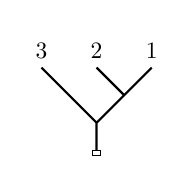
\begin{tikzpicture}[baseline=2ex,scale=0.35,every node/.style={scale=0.85}]
        \clip (-2.5,-0.6) rectangle (2.5,4.45);
        \draw (-0.15,-0.2) rectangle (0.15,0);
        \draw[thick]
            (0,0) -- (0,1) -- (-1,2) -- (-2,3) node[pos=1,above]{$3$}
                    (1,2) -- (0,3) node[pos=1,above]{$2$}
                    (0,1) -- (2,3)  node[pos=1,above]{$1$};
\end{tikzpicture} =
    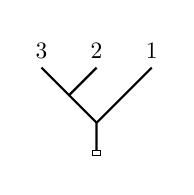
\begin{tikzpicture}[baseline=2ex,scale=0.35,every node/.style={scale=0.85}]
        \clip (-2.5,-0.6) rectangle (2.5,4.45);
        \draw (-0.15,-0.2) rectangle (0.15,0);
        \draw[thick]
            (0,0) -- (0,1) -- (-1,2) -- (-2,3) node[pos=1,above]{$3$}
                              (-1,2) -- (0,3) node[pos=1,above]{$2$}
                    (0,1) -- (2,3)  node[pos=1,above]{$1$};
\end{tikzpicture}
+ 
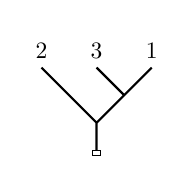
\begin{tikzpicture}[baseline=2ex,scale=0.35,every node/.style={scale=0.85}]
        \clip (-2.5,-0.6) rectangle (2.5,4.45);
        \draw (-0.15,-0.2) rectangle (0.15,0);
        \draw[thick]
            (0,0) -- (0,1) -- (-1,2) -- (-2,3) node[pos=1,above]{$2$}
                    (1,2) -- (0,3) node[pos=1,above]{$3$}
                    (0,1) -- (2,3)  node[pos=1,above]{$1$};
\end{tikzpicture}.
\]
This has origins in the Jacobi relation for the Samelson bracket.

One can prove $(\AS)$ and $(\IHX)$ for the Samelson bracket by imitating the proof that such relations hold for the commutator bracket in the associated graded of the lower central series of a group; see~\cite[Sec.X.5]{Whitehead} for this proof. Note that the relations for the Samelson bracket have graded signs. In particular, the homotopy groups of the wedge sum of $n$ spheres form a free \emph{graded} Lie algebra $\mathbb{L}_n$ on $n$ letters.

Alternatively, one could try to prove that $\realmap_n$ vanishes on \emph{nongraded} $(\AS)$ and $(\IHX)$ directly. For a proof in dimension $d=3$ of a similar result see \cite{CST}. 

The last two paragraphs are not in contradiction, since the subgroup $\Lie_d(n)$ of $\mathbb{L}_n$, consisting of the words in which each letter appears exactly once, is isomorphic to the group $\Lie(n)$ (of nondecorated trees modulo nongraded $(\AS)$ and $(\IHX)$ as in Section~\ref{subsec:trees}), see \cite[Lem.2.3]{K-thesis-paper}. This is also compatible with our inductive definition of Samelson brackets, cf.\ \cite[App.B]{K-thesis-paper}.


Finally, let us discuss some open problems.

    Starting from a connected trivalent graph $\Pi$ on $2n$ vertices Botvinnik and Watanabe~\cite{Botvinnik-Watanabe} constructed a map
    \[
        H^\Pi\colon\S^{n(d-3)}\to\Emb^{\mathrm{fr}}(\S^1\sqcup\S^{d-2},X)
    \]
    where $X$ is any smooth $d$-manifold and the $\S^{d-2}$ component is unknotted and stands still and every $\S^1$ component in the family links it with the linking number one. Thus, they actually have
    \[
        h^\Pi\colon\S^{n(d-3)}\to\Emb^{\mathrm{fr}}(\S^1,X\#\,\S^1\times\ball^{d-1}).
    \]
    since for an unknotted $\S^{d-2}\subseteq X$ we have $X\sm\nu\S^{d-2}\cong X\#\,\S^1\times\ball^{d-1}$. This was stated in \eqref{eq:Botvinnik-Watanabe}.
    
    By attaching $(d+1)$-dimensional $2$- and $1$-handles (dual to $(d-1)$-handles) along these links,  one can associate to $H^\Pi$ an $X$-bundle over $\S^{n(d-3)}$, giving:
    \[
        W(H^\Pi)\colon\S^{n(d-3)}\to B\Diff_\partial(X).
    \]
    Watanabe~\cite{Watanabe} showed using Kontsevich configuration space integrals that the homotopy classes $[W(H^\Pi)]\in\pi_{n(d-3)} B\Diff_\partial(X)$ are nontrivial for $X=\ball^d$ and many $\Pi$.
    \begin{question}\label{quest:Botvinnik-Watanabe}
        How is $h^\Pi$ related to our knotted families?
    \end{question}
    If a direct relation exists, it is bound to give an interesting relation between trivalent graphs on $2n$ vertices and binary trees with $n$ leaves. Moreover, this can give a guiding step for reproving Watanabe's result using embedding calculus.

A natural next step in the geometric study of embedding spaces of $1$-manifolds is the following problem mentioned in Remark~\ref{rem:generalise-all-degrees}.
    \begin{question}\label{quest:real-map-all-deg}
        For each $0<m<d-3$ construct a map
        \[
            \realmap_n^m\colon\pi_{n(d-3)+m}\pF_{n+1}(M)\to\pi_{n(d-3)+m+1}\big(T_n(\D^1,M),\Embp(\D^1,M)\big)
        \]
        such that $\evrel_{n+1}\circ\realmap_n^m=\Id$.
    \end{question}
    
This can probably be done using multi-families that perform embedded commutators of the arcs foliating the meridians, but now allowing more than one use of the same meridian.

Continuing on this is the following problem, which would reprove in the case $C=\D^1$ the fundamental theorem of Goodwillie and Klein \cite{GKmultiple} (see Theorem~\ref{thm:rpn}) by different methods.
\begin{question}\label{quest:reprove-GKW}
    For each $0\leq m<d-3$ prove that $\realmap_n^m\circ\evrel_{n+1}=\Id$ as well.
\end{question}

An easier problem is to try to generalise to all $1$-manifolds, as mentioned in Remark~\ref{rem:nonconn-graspers}:
\begin{question}\label{quest:C-nonconn}
    Does grasper surgery generate $\pi_{n(d-3)}\Embp(C,M)$ also for $C$ nonconnected? Prove the analogue of Theorem~\ref{thm:main} for any $1$-manifold $C$.
\end{question}

    Finally, one can generalise the correspondence of Jacobi and chord diagrams to higher dimensions:
    \begin{question}\label{ques:rel-to-homology}
        How is $\realmap_n$ related to \eqref{eq:Longoni}? Study the exact relation of our classes in homotopy to the classes constructed previously in homology.
    \end{question}



% References
\printbibliography[heading=bibintoc]

\vspace{10pt}
\hrule


\end{document}
